%%% -*-LaTeX-*-

\chapter{Graphs for Data Analysis}
\label{ch:graphs}

% \DPM{Final results to be updated for this chapter.}

\section{The $\beta_p$-Skeleton}
\label{sec:bpskeleton}
Let us begin with a formal definition of the lune-based $\beta$-skeleton.
%
First, we define the open $p$-ball $B$ of radius $r$ centered at some point $c$ in $d$-dimensions to be:

\begin{equation}
\label{eq:ball}
    B_{r,p}(c) = \{x \in \mathbb{R}^d : || x  - c ||_p < r\}
\end{equation}

This is the standard definition of an open ball defined using the $p$-norm.
%
In previous literature, typically $p$ is set to $2$.
%
Given two points $a$ and $b$, their $L^2$ distance $l_{ab}$, and a $\beta$ parameter, we can define a radius $r$ as:
%
\begin{equation}
    \label{eq:beta_radius}
    r =
    \begin{cases}
        \frac{l_{ab}}{2\beta}, & \text{if $0 < \beta < 1$}\\
        \frac{l_{ab}\beta}{2}, & \text{otherwise}.
    \end{cases}
\end{equation}
%
Equation~\ref{eq:beta_radius} allows us to now define the region for the edge $ab$ as follows:
%
\begin{equation}
    R_{\beta,p}(a,b) = \left(\bigcap_{c \in C} B_{r,p}(c)\right)
\end{equation}
%
where $C$ is the set of centers defining the balls:
%
\begin{equation}
C =
\begin{cases}
    \{c \in \mathbb{R}^d: ||a -c||_2 = ||b - c||_2 = r\}, & \text{if $0 < \beta < 1$}\\
    \{(2-\beta)*\frac{a+b}{2} + (\beta-1)*a, (2-\beta)*\frac{a+b}{2} + (\beta-1)*b\}, & \text{otherwise}.
\end{cases}
\end{equation}
%
Formally, we extend the existing empty region definition by considering various $p$ values in Equation~\ref{eq:ball}.
%
Note, $p$ modulates the \emph{shape} of the balls whereas $\beta$ controls the \emph{size} of the balls.
%
The combination of $\beta$ and $p$ allows us to evaluate the performance of an entire spectrum of different values representing graphs we have not seen before in the context of known graphs.

From the definition above, we see that the empty regions of the $\beta$-skeleton can be viewed as the intersection of all balls defined under some metric centered equidistantly from the proposed edge's midpoint.
%
The introduced $p$ parameter defines the $p$-norm to use as the metric.
%
Examples of several different $p$ value shapes are given in Figure~\ref{fig:gabriel_p_shapes} where $\beta$ is assumed to be one.
%
Our generalization allows us to still compute both strict and relaxed versions of our graphs~\cite{CorreaLindstrom2011}.
%
One caveat with our GPU implementation outlined in Section~\ref{sec:gpu_graphs} is that we consider only \textit{symmetric} graphs and not \textit{mutual} versions as defined by Correa and Lindstrom~\cite{CorreaLindstrom2011}.

\begin{figure}[htbp]
    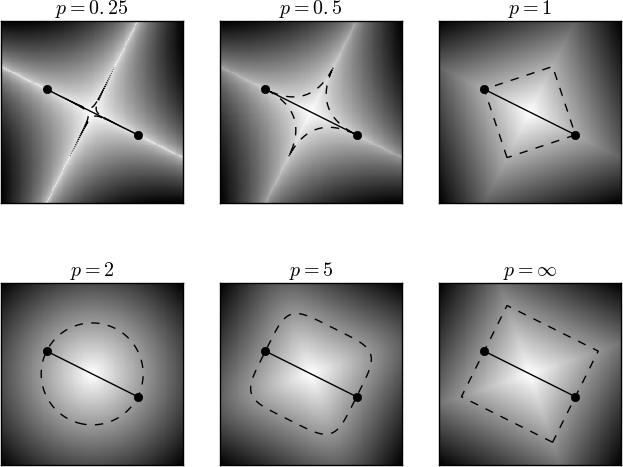
\includegraphics[width=\linewidth]{figs/chap7/emptyRegions}
    \caption[Example $L_p$-norm functions]{The generalization of the Gabriel graph ($\beta$-skeleton where $\beta=1$) using balls defined under different $p$-norms.
    %
    Here we show a graph edge as a solid black line joining two vertices.
    %
    The boundary of the empty region is noted by the dashed line in each example.
    %
    This line is a levelset ($f(c)=1$) of the $p$-norm from the midpoint of the edge.
    %
    The grayscale map denotes this function.
    %
    Note, how the shape of the region varies from a Dirac delta function ($p \rightarrow 0$) to concave to convex to a square in the limit ($p \rightarrow \infty$).}
    \label{fig:gabriel_p_shapes}
\end{figure}

\section{Approximate Cone Graphs for High-Dimensional\\Analysis}

A major challenge of working with cone-based graphs is in the generation of equally sized high-dimensional cones.
%
In order to do this, we first note that we require only the axes of the cones and not the interiors or boundaries.
%
Secondly, the orientation of these cones is not prescribed in any prior work, so any set of uniformly spaced rays emanating from a point will suffice.
%
In order to generate equally spaced cone axes, we utilize a constrained centroidal Voronoi tessellation (CCVT) algorithm to generate approximately equally spaced directions in high dimensions~\cite{DuGunzburgerJu2003}.
%
Specifically, we constrain a CVT sampling to the surface of a $d$-dimensional unit hypersphere.
%
By drawing vectors from the origin to these surface points, we generate a set of roughly equally spaced directions that can be used as the axes of the approximately equally sized hypercones.
%
In our GPU framework introduced in Section~\ref{sec:gpu_graphs}, these directions can be computed once and reused for every point query on the GPU.
%
Alternatively, we can utilize the dependence of the generated directions on the random seed to generate several different realizations.
%
This fact will be exploited in Section~\ref{sec:probabilistic_cones} to create probabilistic cone-based graphs.

Generally speaking, CVTs are known to generate points that represent nearly equal-sized Voronoi
regions~\cite{HesseSloanWomersley2015,PeyreCohen2004}.
%
Given we use a version of Lloyd's relaxation method~\cite{DuGunzburgerJu2003}, which is an iterative method, and we are working in high dimensions, we perform our own study to evaluate the equality of the generated cones where we estimate the surface area of each CCVT sample's Voronoi region on the hypersphere by performing Monte Carlo sampling on the surface of the hypersphere~\cite{HarmanLacko2010,HicksWheeling1959}.
%
By associating every surface point to its nearest site, we can construct a histogram for the sites' count of constituent points.
%
The results are summarized in Figure~\ref{fig:cvt_study}.
%
A two-dimensional example CCVT sample set is shown in the left image with the surface points colored by their membership.
%
The histogram of the middle image shows the frequency of labels for each CCVT site.
%
The black dotted line represent the expected value.
%
The right two line plots summarize our results across dimensions and increasing cone counts.
%
Interestingly enough, we do not see performance degrade as we increase dimensionality, although we do see it degrade as we increase the number of cones.

\begin{figure}[t]
    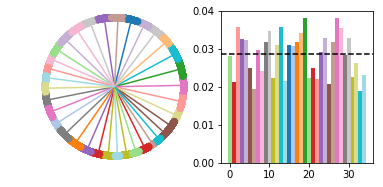
\includegraphics[width=0.65\linewidth]{figs/chap7/cvt_study_35.png}
    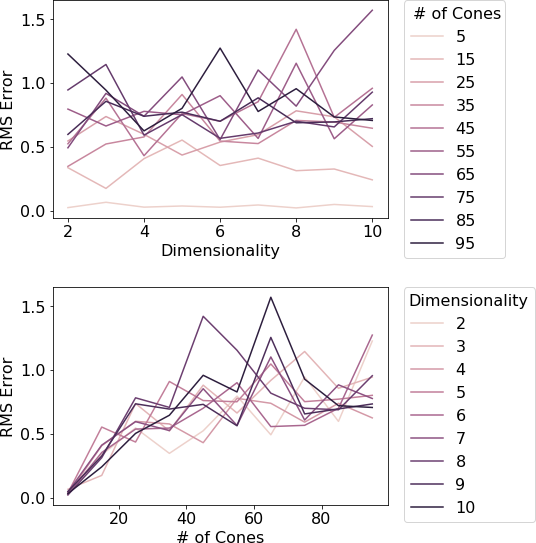
\includegraphics[width=0.32\linewidth]{figs/chap7/scvt.png}
    \caption[Analysis of uniformity from CCVT samples]{A study of the relative areas of constrained CVT samples indicates that their error, although nonzero, is within tolerance for the examples we consider.
    %
    Left: An example CCVT sample showing point membership is used for visual inspection of quality.
    %
    Middle: A histogram showing the membership counts of each site.
    %
    Top right: We summarize the root mean square as a function of the dimensionality.
    %
    Bottom right: We summarize the root mean square error as a function of the number of cones requested.}
    \label{fig:cvt_study}
\end{figure}

% Generally, the number of directions or cones, $c$, should be much smaller than the $k$ value in order to effectively prune redundant directions, but it will also depend on the dimensionality, $d$, of the data.
% %
% This is also advantageous since our approximation is more accurate with smaller values of $c$.

\section{A Unified GPU Framework}
\label{sec:gpu_graphs}

The NGL library~\cite{CorreaLindstrom2011} is an efficient serial implementation able to build $\beta$-skeleton and diamond graphs and their corresponding relaxed versions on arbitrary dimensional datasets.
%
Efficiency is achieved by relaxing the strict requirement of testing all possible edges with all possible points, and thus should be considered an approximation to the true empty region graphs.
%
Even so, the serial implementation of NGL scales only so far on commodity hardware, and as performance improvements are continuously made on the underlying data structures such as the $k$-nearest neighbor graph discussed below, the empty region test remains the bottleneck of this implementation.
%
The GPU-parallel implementation presented here is a simple extension of the technique used by NGL with a few added generalities to allow for the computation of a more robust collection of graphs.
%
In addition, we formulate probabilistic versions of these graphs that are also amenable to the GPU.
%
Our algorithms rely on the same data structures as NGL and thus should be considered approximations to the true graphs.
%
Rather than building graphs incrementally by testing and keeping individual edges, all techniques described from here on will instead prune a supergraph by testing properties of edges in the supergraph and removing those that fail an \emph{edge test} condition.

Both NGL and our proposed method employ an approximate $k$-nearest neighbor ($k$-nn) structure to speed up edge testing.
%
We have built a library that is compatible with several of the leading $k$-nn implementations, as demonstrated in a recent benchmark~\cite{AumullerBernhardssonFaithfull2017}.
%
This benchmark is explored further in Section~\ref{sec:knn_benchmark}, where we also add our own analysis that we believe to be more typical of the use cases under which we consider the $k$-nn graph.
%
Edge testing is limited by considering only edges that exist in the $k$-nn graph.
%
Furthermore, when performing edge tests, we consider only points that are in the $k$-nearest neighborhood of either endpoint.
%
When using this data structure, $k$ is typically set to a large enough value so as to not drastically affect the resulting computation.
%
Again, we comment on how large $k$ needs to be for a typical dataset in Section~\ref{sec:knn_benchmark}.

Let us analyze the amount of storage needed to solve our problem on the GPU as we walk through the algorithm.
%
In this setting, we assume a $k$-nearest neighbor index is available that is able to efficiently return the $k$ nearest neighbors in sorted order for one or more query points in our dataset.
%
Thus far, we have $n \times d$ floating point values representing the locations of a $d$-dimensional point set of size $n$ plus $n \times k$ integers representing the $k$ nearest indices for each of our $n$ points, which must be moved to the GPU for edge validity testing.
%
We then parallelize the pruning operation by associating individual GPU threads to distinct points in the dataset.
%
For each thread/point, we iteratively perform the edge test on each of its neighbors.
%
Thus, each of $n$ threads will perform $k$ edge tests.

For smaller datasets, we can fit the entire $n \times d$ dataset plus its $n \times k$ graph on GPU RAM, and thus we can trivially parallelize the problem using the method described.
%
However, for larger datasets or GPUs with less available memory, we must move part of the problem onto the GPU at a time and process the data in chunks and return the partial, pruned results.
%
Let us consider such a problem, where $b$ is the batch size of points we can process in parallel on the GPU.
%
For simplicity, we utilize a fixed batch size determined by the worst case analysis for the different graphs.
%
In the partial case, we do not want to move the entire point set, but rather only the set of information required for testing.
%
This is where our methodology diverges depending on the graph selected.

For cone-based graphs and relaxed $\beta$-skeletons we need location information only for the points we are pruning and all of their neighbors.
%
In the worst case, each of our $b$ points could each have $k$ distinct neighbors, and thus we require storage of $bkd$ floating point location values.
%
Additionally, we require the indices of the neighboring points mapped to the subset of the location data, which is an additional $bk$ integer index values.
%
From this analysis, we can determine that the largest batch size able to fit into our GPU memory is
%
\begin{equation}
    bkds_{float} + bks_{int} \leq M_{GPU}
\end{equation}
%
where $M_{GPU}$ is the total amount of memory available on our device (in bytes), and $s_{float}$ and $s_{int}$ are the sizes of floats and integers (in bytes), respectively.
%
On the system used for all of the tests performed, we use $s_{float} = s_{int} = 4$.
%
Solving for $b$ results in the following equation,
%
\begin{equation}
    b \leq \frac{M_{GPU}}{k(ds_{float} + s_{int})}.
\end{equation}

The analysis for the strict $\beta$-skeletons requires more storage as we need the locations not only of the points and their neighbors, but also all of their neighbors' neighbors.
%
In the worst case, every neighbor could contribute $k$ points yet unseen in our working subset, resulting in $bkd$ floating point values describing the locations of the query points and all of their neighbors plus an additional $bk^2d$ floating points for the potential $k^2$ neighbors of neighbors.
%
Additionally, we require storing mapped integer indices to this subset of data to represent the neighborhoods.
%
In this case, we have $b$ query points with $k$ neighbors each plus we need the $k$ neighbors of each of those neighbors.
%
The result is $b(k + k^2)$ integer values.
%
In summary, the available batch size for the strict $\beta$-skeletons on a device with $M_{GPU}$ bytes of free memory is given below,
%
\begin{equation}
    b \leq \frac{M_{GPU}}{(k+k^2)\left(ds_{float} + s_{int}\right)}.
\end{equation}
%
This memory footprint affords much less parallelism, and one should consider moving to an adaptive batch-sizing scheme and/or possibly sorting data points based on their location in order to batch nearby query points together to avoid this worst-case upper bound when using the strict $\beta$-skeleton for very large datasets.
%
% We instead focus our attention on comparing the relative performance of the relaxed and strict versions algorithm in order to make a case that for many practical purposes the relaxed $\beta$-skeletons are ``good enough.''

% \dpm{For our $6$GB test machine working up to $5$D with a $k=1024$ and assuming $s_{float} = s_{int} = 4$, we can still achieve parallelism with a batch size of $238$, however with a relaxed $\beta$-skeleton or a cone-graph we can achieve $b=244140$}

\subsection{Empty Region Graphs}
We begin with an observation that the empty region shapes defined by any particular $\beta_p$-skeleton are symmetric in all directions orthogonal to an edge regardless of the dimensionality of the embedding space of the edge.
%
Thus, we can reduce all point-in-empty-region tests to a one-dimensional problem.
%
We accomplish this reduction by defining the edge as a vector, say from point $a$ to point $b$.
%
We then form vectors to every $k$ nearest neighbor, $q$, of $a$ (and $b$, if computing the strict version of the graph).
%
Every vector $aq$ is projected onto $ab$ using a dot product that yields a parameterization of $t_q$.
%
The maximal shape any lune-based $\beta_p$-skeleton can attain is the infinite slab of space bounded by two hyperplanes, each one intersecting one endpoint and perpendicular to the edge.
%
An example of this region is shown by the shaded region in the left image of Figure~\ref{fig:infinite_slab} for the two-dimensional case.
%
The upper limit of this shape implies that only points that have $t$ value on the range $(0,1)$ can possibly intersect the empty region.
%
For the neighbors whose $t_q \in (0,1)$, we compute the $L^2$-norm from $q$ to the edge and compare it with the empty region.

\begin{figure}[b]
    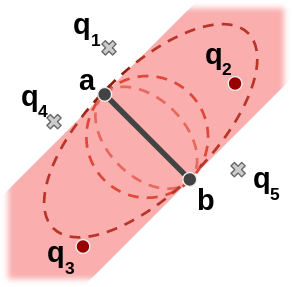
\includegraphics[width=0.34\linewidth]{figs/chap7/infinite_slab.png}
    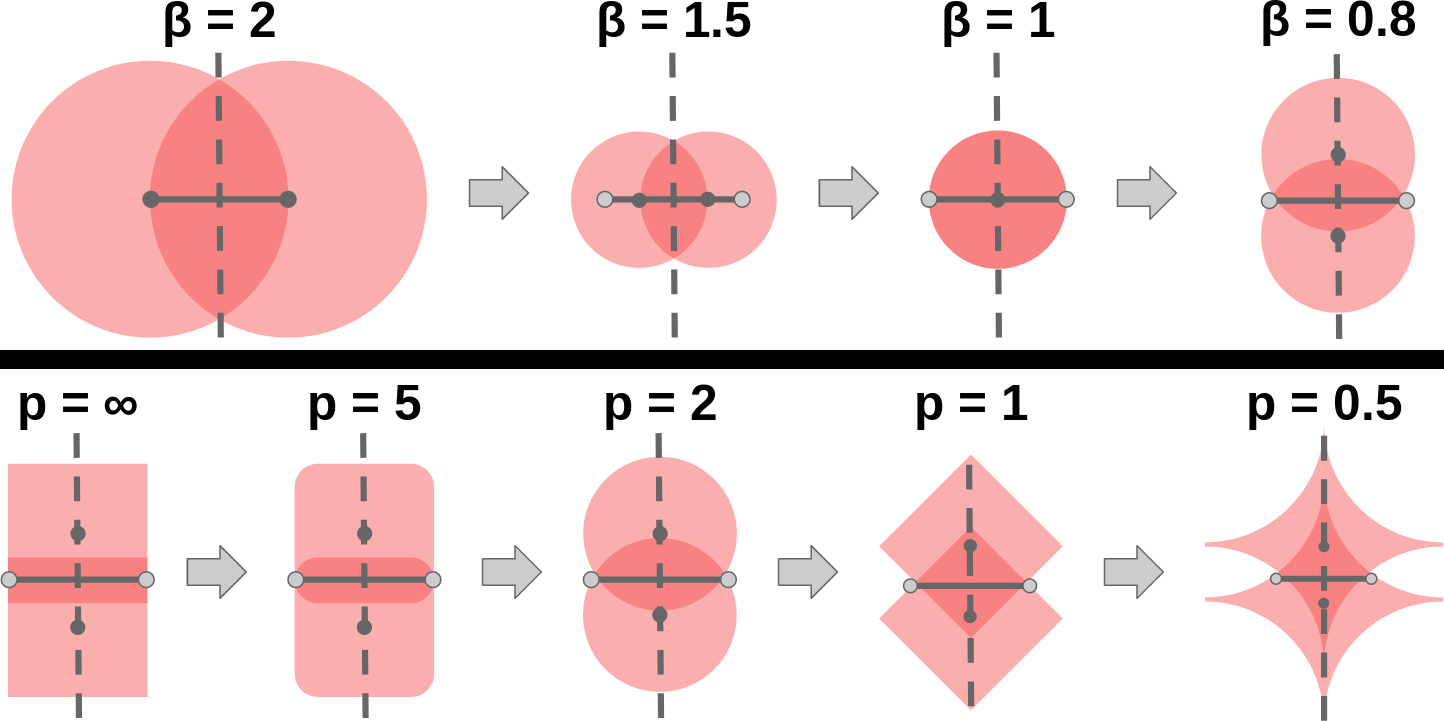
\includegraphics[width=0.64\linewidth]{figs/chap7/variable_parameters.png}
    \caption[Illustration of various $\beta_p$-skeleton shapes]{Left: Consider an edge between points $a$ and $b$ and neighbors to $a$, $q_{i}$.
    %
    The shaded region represents $R$ for the infinite slab graph ($p < 1, \beta \rightarrow 0$).
    %
    All other parameterizations of the $\beta_p$-skeleton will yield subsets of this region.
    %
    Dotted curves represent the empty regions of other parameterizations.
    %
    Thus, $q_{1,4,5}$ do not need to be tested since they fall outside this slab.
    %
    $q_2$ and $q_3$ may violate the empty region property depending on the values of $p$ and $\beta$.
    %
    Right: We show how $\beta$ and $p$ separately affect the shape of $R$ in two dimensions.}
    \label{fig:infinite_slab}
\end{figure}

We now shift our attention to the empty region and how it can be represented as a scalar function defined from either endpoint to the edge's midpoint.
%
Note, we assume the empty region is symmetric about the proposed edge's midpoint, which satisfies the undirected condition, $R_{\beta,p}(a,b)=R_{\beta,p}(b,a)$.
%
Therefore, we can parameterize the minimum allowable distance to an edge as a function of how far along the edge we are in one dimension by properly distancing one $p$-ball appropriately from the edge's midpoint.
%
Given $u \in [0, 1)$ as the parameterization of a point's distance from the edge midpoint, we can define the minimum allowable distance of the $\beta_p$-skeleton as follows:
%
\begin{equation}
    \label{eq:beta_parameterization}
    D(u) = \sqrt[p]{r^{p} - (u - c_x)^p} - \sqrt[p]{c_y}
\end{equation}
%
where $r$ is the radius of a two-dimensional $p$-ball defined by Equation~\ref{eq:beta_radius} and $c$ is the center of said ball with position defined by:
%
\begin{equation}
    c =
    \begin{cases}
        \left(0, \beta^{-p} - 1\right), & \text{if $0 < \beta < 1$}.\\
       \left(1-\beta, 0\right), & \text{otherwise}.
    \end{cases}
\end{equation}
%
Figure~\ref{fig:beta_p_example} shows an example edge test for a two-dimensional case.
%
In the left image, we see how the points are arranged in the input space.
%
In the right image, the point $q$ is shown parameterized along the edge $ab$.

\begin{figure}[b]
    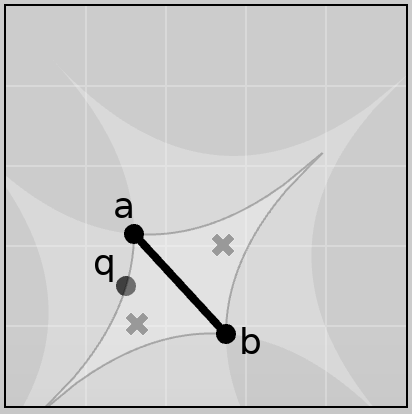
\includegraphics[width=0.48\linewidth]{figs/chap7/bskeleton.png}
    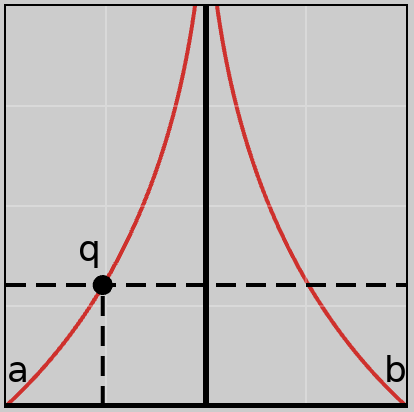
\includegraphics[width=0.48\linewidth]{figs/chap7/bskeletonParameter.png}
    \caption[Illustration of the one-dimensional edge test]{Left: An example of a two-dimensional edge defined by points $a$ and $b$.
    %
    We test whether the query point $q$ is interior to the region $R_{\beta,p}(a,b)$.
    %
    $R_{\beta,p}(a,b)$ is defined as the intersection of two $p$-balls whose center points are shown as gray x's.
    %
    Right: The edge test can be reformulated as a 1-dimensional problem where we compare $q$'s $L^2$-distance to $ab$ and the equation of the $p$-ball centered at a distance determined by $\beta$ from the edge's midpoint.}
    \label{fig:beta_p_example}
\end{figure}

\subsubsection{Discretized Empty Region Graph Algorithm}
\label{sec:gpu_bp_discrete}

The one-dimensional function given in Equation~\ref{eq:beta_parameterization} has only one dependence on the length of $ab$.
%
Thus, we can precompute the template function offline and scale it accordingly for each edge in our GPU kernel.
%
The result is a discretized algorithm where the fidelity of the precomputed approximation is a function of the number of discrete steps $s$ used to store the function.
%
Note, since the function is symmetric about the midpoint, we can devote all $s$ samples to one half of the shape, as noted by the domain of Equation~\ref{eq:beta_parameterization}.

Furthermore, this simplification allows us to substitute any arbitrarily complex kernel function for the $L^p$-balls presented thus far.
%
For example, in Figure~\ref{fig:discrete_beta}, we demonstrate the use of a several different common kernel functions, including a properly scaled Gaussian, Epanechnikov, cosine, quartic, and tricubic functions on a set of 20 CVT sampled points in two dimensions.
%
We compare these results with the standard $L^p$ norm example and note that the results are unique for each realized graph.
%
This generalization allows for much more flexibility in designing an optimal graph for a specific problem, and the merits of using different kernel shapes require further investigation.

\begin{figure}[htbp]
    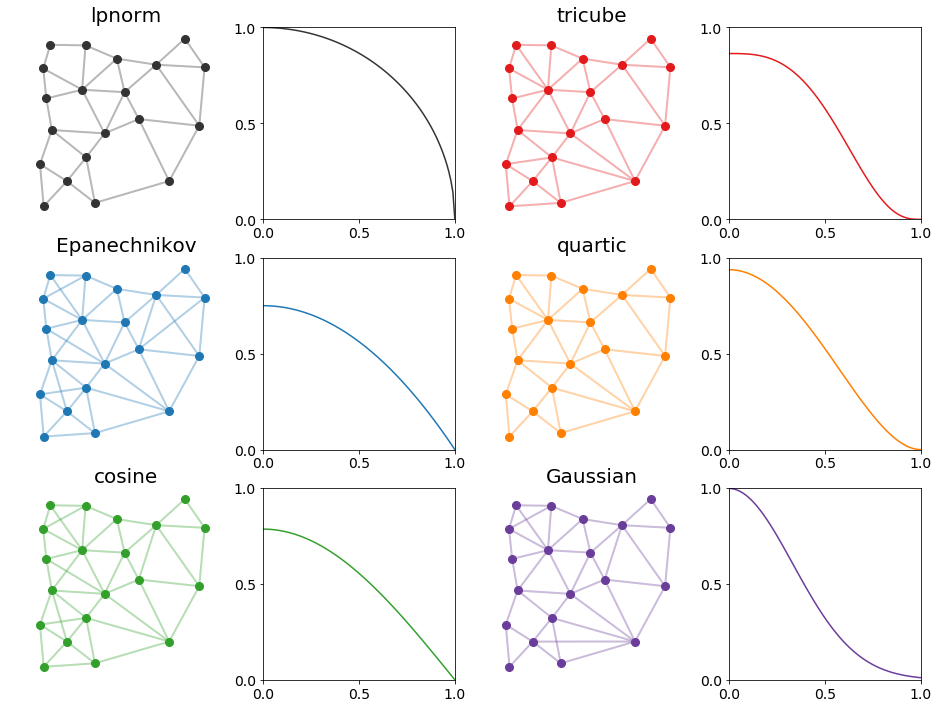
\includegraphics[width=\linewidth]{figs/chap7/beta_shapes.png}
    \caption[Empty region graphs derived using kernel functions]{Using discretization to precompute a template function, we can employ arbitrarily complex functions without incurring any additional overhead cost.
    %
    Here we demonstrate using several different common kernel functions and visual the resulting graph.
    %
    The color-coordinated adjacent line plots of each graph show the shape of the template functions used.}
    \label{fig:discrete_beta}
\end{figure}

\subsubsection{Probabilistic Empty Region Graphs}

Here we introduce a modified method for computing probabilistic $\beta_p$-skeletons that is similar in spirit to the methodology used by Correa and Lindstrom's stochastic empty region graph.
%
Both methods relate an edge's probability to the largest minimum distance any empty-region-violating point needs to move to be placed outside of an edge's empty region.
%
We differ in how we parameterize the problem.
%
Both methods are equally applicable within our GPU framework.

Correa and Lindstrom utilize an inner and outermost region $R_{\alpha_{min}}$ and $R_{\alpha_{max}}$, where probability uniformly increases from 0 to 1 for $\alpha \in [\alpha_{min},\alpha_{max}]$ over this region.
%
Any edge with a neighbor inside $R_{\alpha_{min}}$ will have probability 0, and any edge with no neighbors inside of $R_{\alpha_{max}}$ will have probability 1.
%
We instead utilize a logistic function~\cite{Cramer2002} in order to adjust the steepness of the probability fall-off and do not express set minimum and maximum regions.
%
Given a neighbor $q$'s projection onto $ab$, $t_q$, its $L^2$ distance from $ab$, $d_{t_q}$, and $D(\cdot)$ from Equation~\ref{eq:beta_parameterization}, we define an edge's probability with respect to $q$ as:
%
\begin{equation}
\label{eq:probabilistic_beta}
    l(t_q) = \left(1 + e^{-\frac{k\left(d_{t_q}-r\right)}{r}}\right)^{-1}
\end{equation}
%
where $r = D(2|t_q - 0.5|)$ and $k$ is a free parameter defining the steepness of the function.
%
In other words, a large $k$ means the probability will go from 0 to 1 in a very small region about the reference shape, whereas a low value of $k$ will stretch the probability ramp up over a larger area in both directions about the reference shape.
%
Thus, the probability of an edge is the minimum of Equation~\ref{eq:probabilistic_beta} for all neighbors considered for an edge's endpoints.
%
The method employed by Correa and Lindstrom has the nice property of having hard cut-off points for the probability and using a linear ramp within it.
%
The logistic function proposed here gives the user more control on the shape of the probability function at the expense of losing strict boundaries, although one could employ hard bounds to this function if desired.
%
We can modulate the steepness through a parameter $k$, and the probability ramp is no longer linear, but instead an s-shaped curve.
%
The point here is to demonstrate here the probability can be formulated using any monotonic function and could vary depending on the demands of the specific application.

An example probabilistic graph is shown in the rightmost image of Figure~\ref{fig:probabilistic_beta}.
%
The leftmost plot shows the shape of the specific logistic function, and the center image shows the probability as a function of distance from a specific edge.
%
In the right image, solid lines represent probability above $75\%$, dashed-dotted lines represent probability above $50\%$, dashed lines represent probability above $25\%$, and dotted lines represent edges with $<25\%$ probability.

\begin{figure}[htbp]
    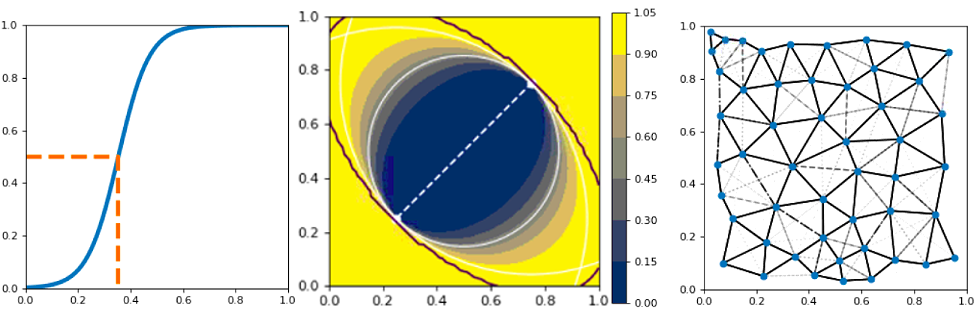
\includegraphics[width=\linewidth]{figs/chap7/probabilistic_beta.png}
    \caption[Example computation of probabilistic Gabriel graph]{An example of a probabilistic Gabriel graph.
    %
    The left plot shows the logistic function used to determine the steepness by which the probability will fall off as a distance from the canonical empty region boundary (in this case the white circle of the middle image).
    %
    The orange line indicates the 50\% probability point, which aligns with the reference shape, which is the white circle in the middle image in this case.
    %
    The middle image shows the probability as a colormap under the edge.
    %
    The right image visualizes the graph using different line styles to denote probability.
    %
    Solid lines $>75\%$, dashed-dotted lines $>50\%$, dashed $>25\%$, dotted $\leq25\%$.}
    \label{fig:probabilistic_beta}
\end{figure}

\subsection{Cone Graphs}

Consider that we want to compute either an $m$-Yao or $m$-$\Theta$-Graph where $m$ is the number of points per cone.
%
For a given query point, we initialize a counting array of size $c$ zeros.
%
We then iteratively compute the $i$th nearest neighbor's cosine similarity to each of the $c$ axes and determine which cone this neighbor belongs to by taking the maximum.
%
Cosine similarity measures the directional similarity of two vectors by computing the cosine of the angle between them, thus a value of 1 means the vectors are in the same direction and a value of -1 means they are in opposite directions.
%
The value can be computed by performing a dot product between the two normalized vectors.
%
If the counting array index associated to this cone is less than $m$, we increment the count and keep this edge.
%
Otherwise, we invalidate this edge by replacing it with a $-1$.
%
For the Yao graph, we make use of the ordered $k$-nearest neighbors provided by our $k$-nn query structure.
%
Since the $k$-nearest neighbors for each point are given in order of increasing distance to the query point, we are guaranteed to fill each conic with the the closest neighbors first for the Yao graph.

If instead we are computing the $\Theta$ graph, we must reorder the points based on their projected distance, which we have already computed in order to determine the closest axis.
%
Alternatively, we could use an auxiliary data structure to maintain the $m$ closest distances for each axis and process the neighbors sequentially.
%
Thus, we can incur a $\bigO(k \log k)$ sort operation per query point/thread to sort the $k$ neighbors in increasing distance to their respective axis, or add a local $\bigO(cm)$ storage per thread to store the $m$ closest distances for each of the $c$.
%
For most practical settings, $m$ is set to 1 or 2 and we seek to use a minimal $c$ that achieves the fidelity we want, whereas $k$ is often maximized in order to start with the most information possible for pruning.
%
These observations would seem to favor the latter methodology, however the sorts can be done in parallel for each query.
%
% We examine both implementations in Section~\ref{exp:performance}.
% %
% \dpm{I have not implemented this. Make sure there are no devils in the details.}

\subsubsection{Probabilistic Cone Graphs}
\label{sec:probabilistic_cones}

Note that the resulting edges from the cone graphs are largely dependent on the generated directions used for the cone axes.
% %
% The $\Theta$-graph especially can select a completely different set of neighbors with only a small perturbation in angle of directions.
% %
% Figure~\ref{fig:cone_graphs} demonstrates how rotating the axes with the same point set yields different results for both the Yao and $\Theta$-graph.
% %
% In this case, two of eight Yao neighbors have changed, and seven of
% eight $\Theta$ neighbors have changed.
%
Exploiting this fact, one way to generate a probabilistic result is to use several different random seeds for the CCVT sample generation.
%
The result is a collection of different graph realizations.
%
We then associate probability to an edge equal to the proportion of realizations in which it occurs.
%
The justification for doing this is that stable edges will be robust to the actual cones selected.

% \begin{figure}[htbp]
%     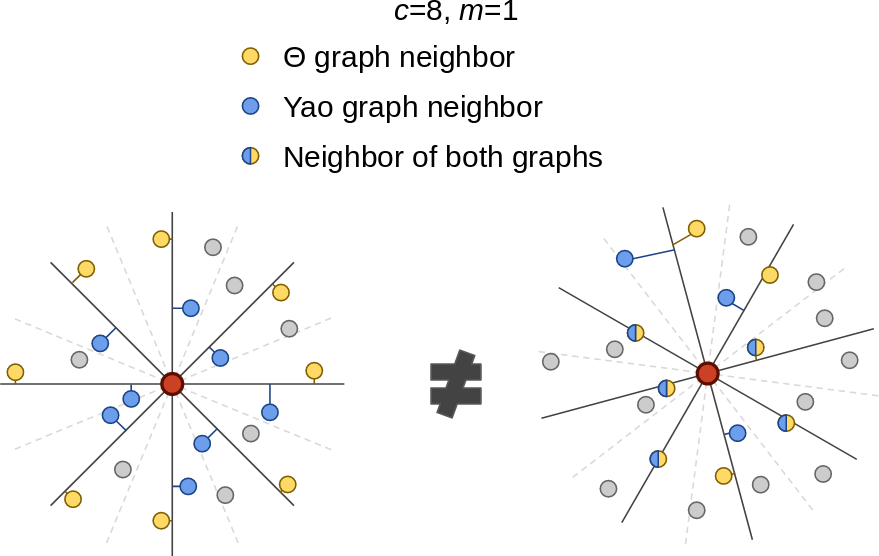
\includegraphics[width=\linewidth]{figs/chap7/cone_graphs.png}
%     \caption{Two examples are shown for determining neighbors of the
%     same central red query point.
%     The solid lines represent the $8$ cone axes which are perturbed
%     between the two images. Blue and yellow dots represent neighbors
%     identified by the Yao and $\Theta$ graphs, respectively. Dotted
%     lines represent cone boundaries and gray points are points that
%     are not neighbors to the query point under either graph
%     representation. \dpm{Re-do this image with corrected $\theta$ graph.}}
%     \label{fig:cone_graphs}
% \end{figure}

\section{Quality Measures}
\label{sec:graph_quality_measures}
An open question to consider is what makes a ``good'' graph?
%
Although the answer largely depends on the application, we attempt to generalize properties from the topological and geometric properties of the dataset as well as our target applications and come up with five measures applicable in low dimensions to evaluate different proximity graphs.
%
For higher dimensions, we will rely on an application-specific studies to evaluate performance.

The five measures are listed below with a brief justification for each.
%
These five measures capture the consistency in topology and geometry between the graph and the underlying data distribution.
%
Two of the quality measures are computed from the properties of the graph, and the remaining three rely on both the constructed graph and the computation of an $\alpha$-shape~\cite{EdelsbrunnerKirkpatrickSeidel1983}, where we tune $\alpha$ for each chosen dataset in order to extract a tight hull of the distribution of points in the plane.
%
Examples of the point distributions evaluated and their extracted alpha shapes are given in Figure~\ref{fig:shapes}.

\begin{figure}[htbp]
    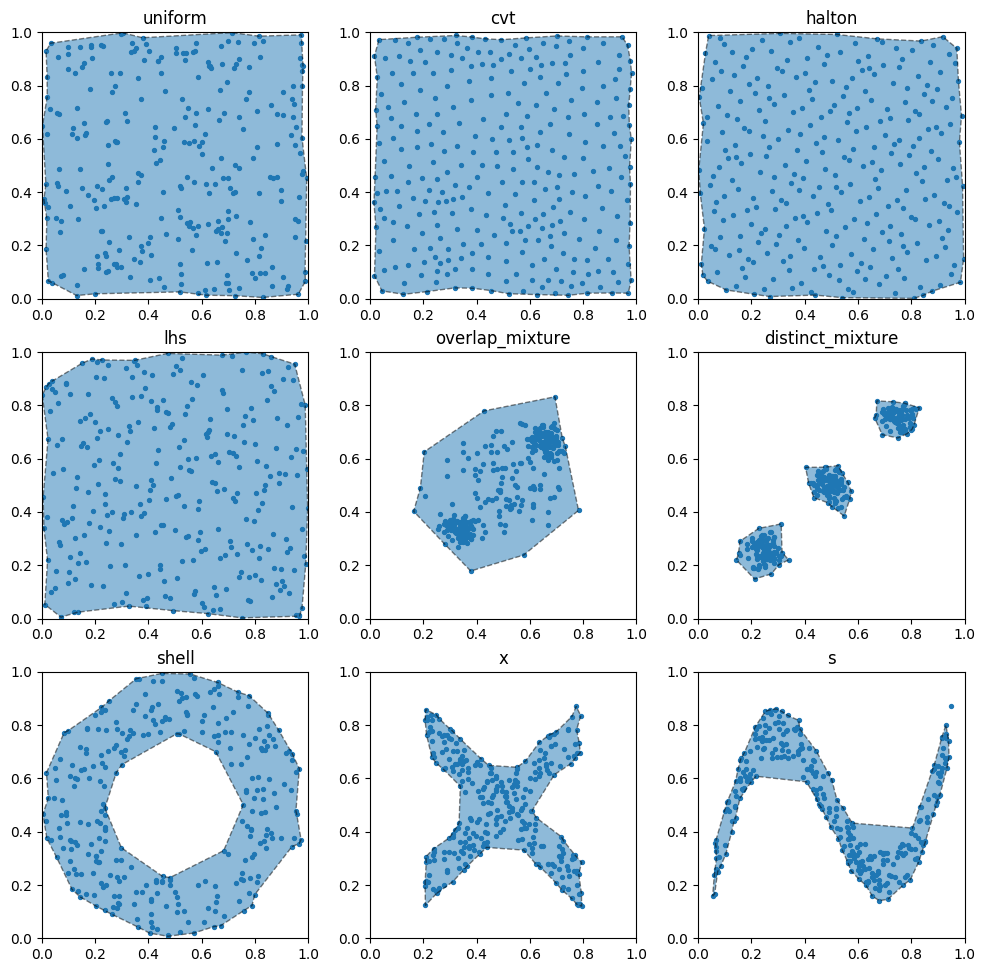
\includegraphics[width=\linewidth]{figs/chap7/sample_shapes.png}
    \caption[$\alpha$-shapes of the two-dimensional distributions used for graph quality study]{Two-dimensional point distributions used for our graph quality analysis and their $\alpha$-shapes.}
    \label{fig:shapes}
\end{figure}

\subsection{Crossing Edge Count}
%
Crossing edges encode redundant information by overconnecting the graph and can actually create contradictory information in terms of interpolation.
%
For example, in the application of scalar field topology, the presence of crossing edges can result in crossing integral lines, which violates one of the fundamental tenets for analysis.
%
The number of crossing edges is computed and used as a negative measure in building a good graph.

\subsection{Average Induced Polygon Area}
%
If crossing edges represent an overconnected graph, then the amount of empty space represents the other side of the spectrum, an underconnected graph.
%
One way to compute the amount of empty space in a graph is to induce a polygonization of the graph by including all faces where the edges of our graph form a closed polygon.
%
By computing the average area of this set of polygons, we get a sense of how much empty space there is in the graph's interior.
%
The larger the area of the polygons, the more prone the graph is to being sparse.
%
The problem with this measure in isolation is that it will tend to favor underconnected graphs that have no closed polygons and so will report a minimal value of zero for the average area.
%
We counterbalance this measure with the number of crossing edges and the next measure, which ensures the topological consistency.

\subsection{Connected Components}
%
We compute the absolute difference between the number of connected components of the alpha shape and the number of connected components of the graph.
%
By verifying the number of connected components, we will penalize both underconnected graphs, which create many small and spurious components, and overconnected graphs, which fail to capture the intrinsic shape of the data.

\subsection{$\alpha$-shape Coverage}
%
Using the induced polygonization from above, we can also compute how well that polygonization covers the shape of the data.
%
For this computation, we perform an intersection operation between the induced polygonization and the $\alpha$-shape.
%
We then compute the total area of this intersection divided by the total area of the $\alpha$-shape.
%
In this way, a value of 1 represents complete coverage of the shape and a value of 0 means no coverage.

\subsection{Total Out-of-bounds Length}
%
To compensate for the previous measure, where a fully connected graph will always report a coverage of 1, we also compute the lengths of edges outside the $\alpha$-shape.
%
% The problem with the previous measure is that a fully connected graph will always report a coverage of one.
%
The coverage measure can in some sense be thought of as a recall measure, showing how much of the total shape of the data can be recovered.
%
Naturally, it would make sense to couple that with a precision measure that penalizes edges that fall outside of the $\alpha$-shape.
%
To satisfy this criterion, we chose to accumulate the total length of edges outside the $\alpha$-shape.
%
We perform a difference operator on all edges, such that we include only the portions of edges that fall outside of the given $\alpha$-shape.

\subsection{Composite Measure}
In order to digest these five measures, we normalize them over their respective ranges and perform linear scalarization~\cite{HwangMasud1979} to create a composite measure that we can use to optimize the parameters of each graph type,

\begin{equation}
    M_{composite} = \sum_{i=1}^5 M_iw_i.
\label{eq:composite_measure}
\end{equation}

For the experiments in this chapter we use $w_i=1$.
%
For all but one of our measures a lower value is better.
%
The $\alpha$-shape coverage is the one exception where a higher value yields a more desirable graph.
%
Therefore, in addition to scaling all the values, we also negate the $\alpha$-shape coverage before computing the sum in Equation~\ref{eq:composite_measure}.
%
Thus, the most desirable graph from our analysis will have the lowest composite quality measure.

\section{Analysis}

The remainder of this chapter enumerates a series of experiments to evaluate various aspects of these graphs in context.
%
We begin with a study on the $k$-nn graphs evaluating the performance of various available implementations in the context of computing extremum graphs~\cite{CorreaLindstromBremer2011} in moderate dimensionality.
%
Next, we investigate the proper selection of $k$ to ensure we reach the \textit{saturation point} for a relaxed Gabriel graph, that is, where all of the true edges of the requested graph are part of the original $k$-nearest neighbor query result.
%
In other words, we identify the minimum value of $k$ that yields a recall of 1 for the true relaxed empty region graph.
%
Then, we evaluate the speed of our GPU implementation compared with the existing NGL library.
%
Finally, we compare the traits of $k$-nn graphs, empty region graphs, and cone graphs in three tests.
%
The first uses our quality measures defined in Section~\ref{sec:graph_quality_measures}, the next seeks to determine the topological stability imposed by different graphs, and the last we apply these graphs to the classification algorithm.

\subsection{$K$-NN Comparison}
\label{sec:knn_benchmark}

With the speed-up from performing the empty region tests on the GPU, the runtime should be dominated by the neighborhood queries.
%
There exist a number of publicly accessible libraries for efficiently calculating $k$-nn graphs and query structures.
%
The ann-benchmark~\cite{AumullerBernhardssonFaithfull2018} has been used to evaluate nearly 20 algorithms on typical datasets.
%
However, many of these algorithms are designed to exploit largely empty spaces where the data is expected to lie on a manifold of intrinsic dimensionality significantly smaller than the extrinsic dimension $d$, and the benchmark data is chosen accordingly.
%
On the contrary, in many science and engineering applications, datasets often represent ensembles of simulations designed to explore a parameter space scaled to be the unit-hypercube $[0,1]^d$.
%
These types of point distributions lead to different query characteristics and challenges.
%
Here, we provide an extension to this benchmark using uniform samples of two- to five-dimensional hypercubes with 1-10 million points.
%
In addition, we performed our own analysis that uses each of these libraries as a precursor for pruning the relaxed Gabriel graph and subsequently computing an extremum graph using the streaming algorithm discussed in Section~\ref{sec:extremumGraph} and Liu et al.~\cite{LiuWangMaljovec2019}.
%
All results were generated on a machine equipped with a Intel Core i7-6700 CPU, 16 GB of RAM, an Nvidia GeForce 980 Ti GPU, and 6GB of VRAM.

A sample result of using ann-benchmark on our generated data is shown in Figure~\ref{fig:pareto} where each colored line represents the empirical Pareto front of an individual algorithm over a sample set of various algorithmic parameters trading off accuracy (horizontal axis, right is more accurate) and speed (vertical axis, higher is faster).
%
This benchmark highlights the best possible performance, but is not indicative of actual performance on large data where parameter tuning may be infeasible.
%
Additionally, this benchmark does not include the time needed to build the query structure, presumably because these structures are used over long periods of time or replicated across distributed devices, and the preprocessing time is amortized over the life of the structure.
%
In our case, preprocessing time represents a significant portion of the computation, since the lifetime of our $k$-nearest neighbor structure is much more transient.
%
We do not need the $k$-nn structure once we have computed our approximate proximity graph.
%
Thus, we perform additional analysis where parameters are set to default values or when not default values are not available, we choose to favor speed over accuracy, and where build time is included in the analysis.

\begin{figure}[t]
    \centering
      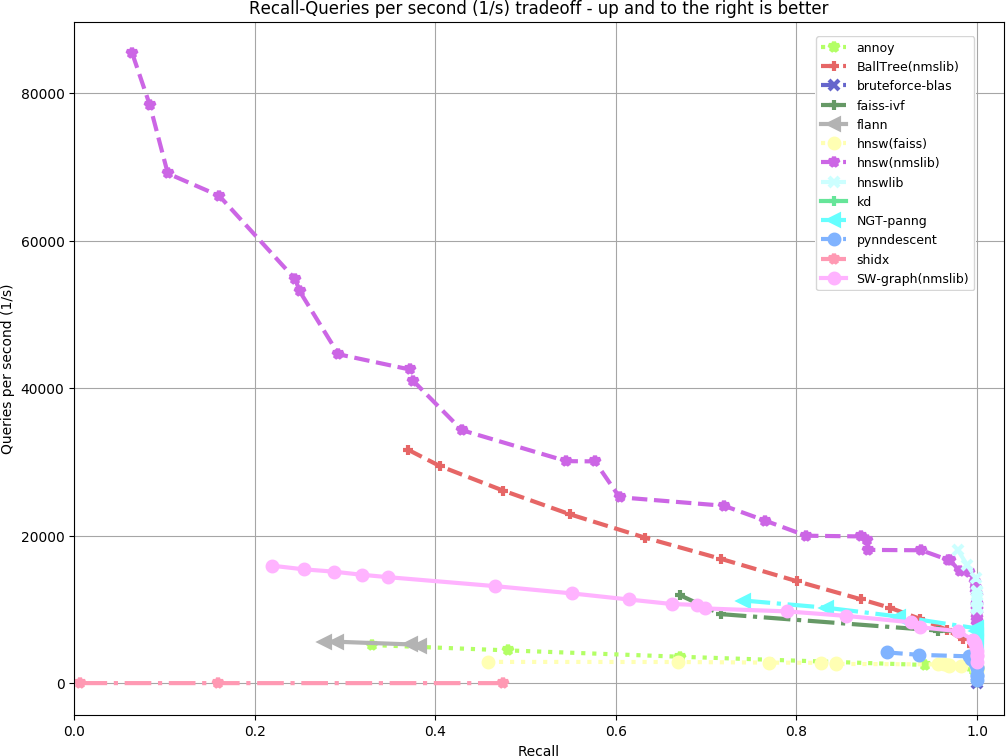
\includegraphics[width=.95\linewidth]{figs/chap7/uniform-5-euclidean.png}
     \caption[Example performance plot generated by ann-benchmarks]{Pareto front of Various ANN implementations trading off accuracy vs.
       speed on a 1 million point set in 5D under different parameter settings.
       %
       The data was sampled using a uniform random strategy so the domain should be
       considered to be more evenly and densely sampled in this benchmark as
       opposed to those provided in the study of Aum{\"{u}}ller et
       al.~\cite{AumullerBernhardssonFaithfull2018}.
       %
       The horizontal axis represents the ability of the algorithm to recall the
       correct $k$ nearest neighbors of the graph for each point.
       %
       The vertical axis is the number of queries able to  processed per second.
       %
       This graph was generated by ann-benchmarks~\cite{ANNBenchmark}.
     }
    \label{fig:pareto}
\end{figure}

As we can see in Figure~\ref{fig:knn_benchmark}, which shows actual timings when each algorithm is used in our pipeline, results vary in practice.
%
In this set of tests, we are querying much larger $k$ values that will be pruned heavily.
%
For this reason, we prioritize speed over accuracy in many of the approximate algorithms, with the exception of ANN, FLANN, and FAISS, where we are able to compute exact results.
%
We also exploit GPU and OpenMP parallelism where applicable.
%
Despite being an exact solution, the OpenMP version of FLANN, which is used to construct the exact $k$-nearest neighbor graph, is able to outperform many of the approximate algorithms in our dense cases.
%
However, if the entire $k$-nearest neighbor graph can fit in memory or multiple GPUs can be exploited, the FAISS-GPU algorithm may be preferred because it will not need to share GPU memory with the pruning phase.
%
Otherwise, as is the case in our example, the $k$-nn search index must be deallocated and reconstructed after each batch of pruning in order to free memory for the GPU-based pruning phase.

\begin{figure}[t]
    \centering
      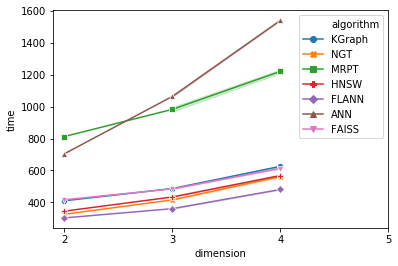
\includegraphics[width=.95\linewidth]{figs/chap7/relaxed_gabriel_benchmark_1M.png}
    \caption[Custom benchmark performance for various $k$-nn implementations]{Average execution times of our code's ability to prune a
    $k$-nearest neighbor graph of one million points in varying dimensions
    to a relaxed Gabriel graph using various approximate KNN libraries.
    %
    For all examples, $k=1024$, averages are reported over five trials
    of different random, uniform point sets; graph pruning is done
    in batches of one hundred thousand points; and results have been
    validated against a true relaxed Gabriel graph on the same datasets.
    %
    All results are within an acceptable tolerance of error.
  }
  \label{fig:knn_benchmark}
\end{figure}

\subsection{$\beta$-Skeleton Saturation Point}

We define the \textit{saturation point} of one of our pruned graphs as the minimum $k$ value needed to make our approximate graph equal to the true graph we are attempting to replicate.
%
For this section, we perform an experiment using a relaxed Gabriel graph as our test graph.
%
To determine a suitable $k$, we gradually increase $k$ in the initial $k$-nearest neighborhood query stage and observe at which point the number of edges of the empty region graph starts to stabilize.
%
Results are presented in Figure~\ref{fig:graph_degree}.
%
We can see from the image on the right that in this five-dimensional space, the curve starts to level off beyond $k\sim500$, indicating that adding more $k$ neighbors will not result in many more edges being discovered in the pruned graph.
%
The saturation point will vary based on the distribution of the data in the domain.
%
The results are shown for data drawn from a uniform random distribution.

Additionally, in the same figure, we construct a histogram of the degrees of every point in the data.
%
This histogram demonstrates that even in five dimensions the relaxed Gabriel graph of a dense sample results in an average of $\approx35$ edges per vertex, which, for the largest example in the studies of Liu et al.~\cite{LiuWangMaljovec2019} reaches 10 million points, results in roughly 350 million edges.
%
Assuming 64-bit indices, this size of graph results in over 40GB of storage compared to the 1.7GB necessary for the vertex information (5+1 32-bit floats for the domain and range of the function).
%
In principle, the graph storage can be reduced to 20GB since, in a symmetric graph, we need to store only one ``direction'' of an edge and process the other one implicitly.
%
This analysis demonstrates the need for the streaming computation of these graphs for applications like those in Liu et al.~\cite{LiuWangMaljovec2019}.

\begin{figure}[t]
    \centering
      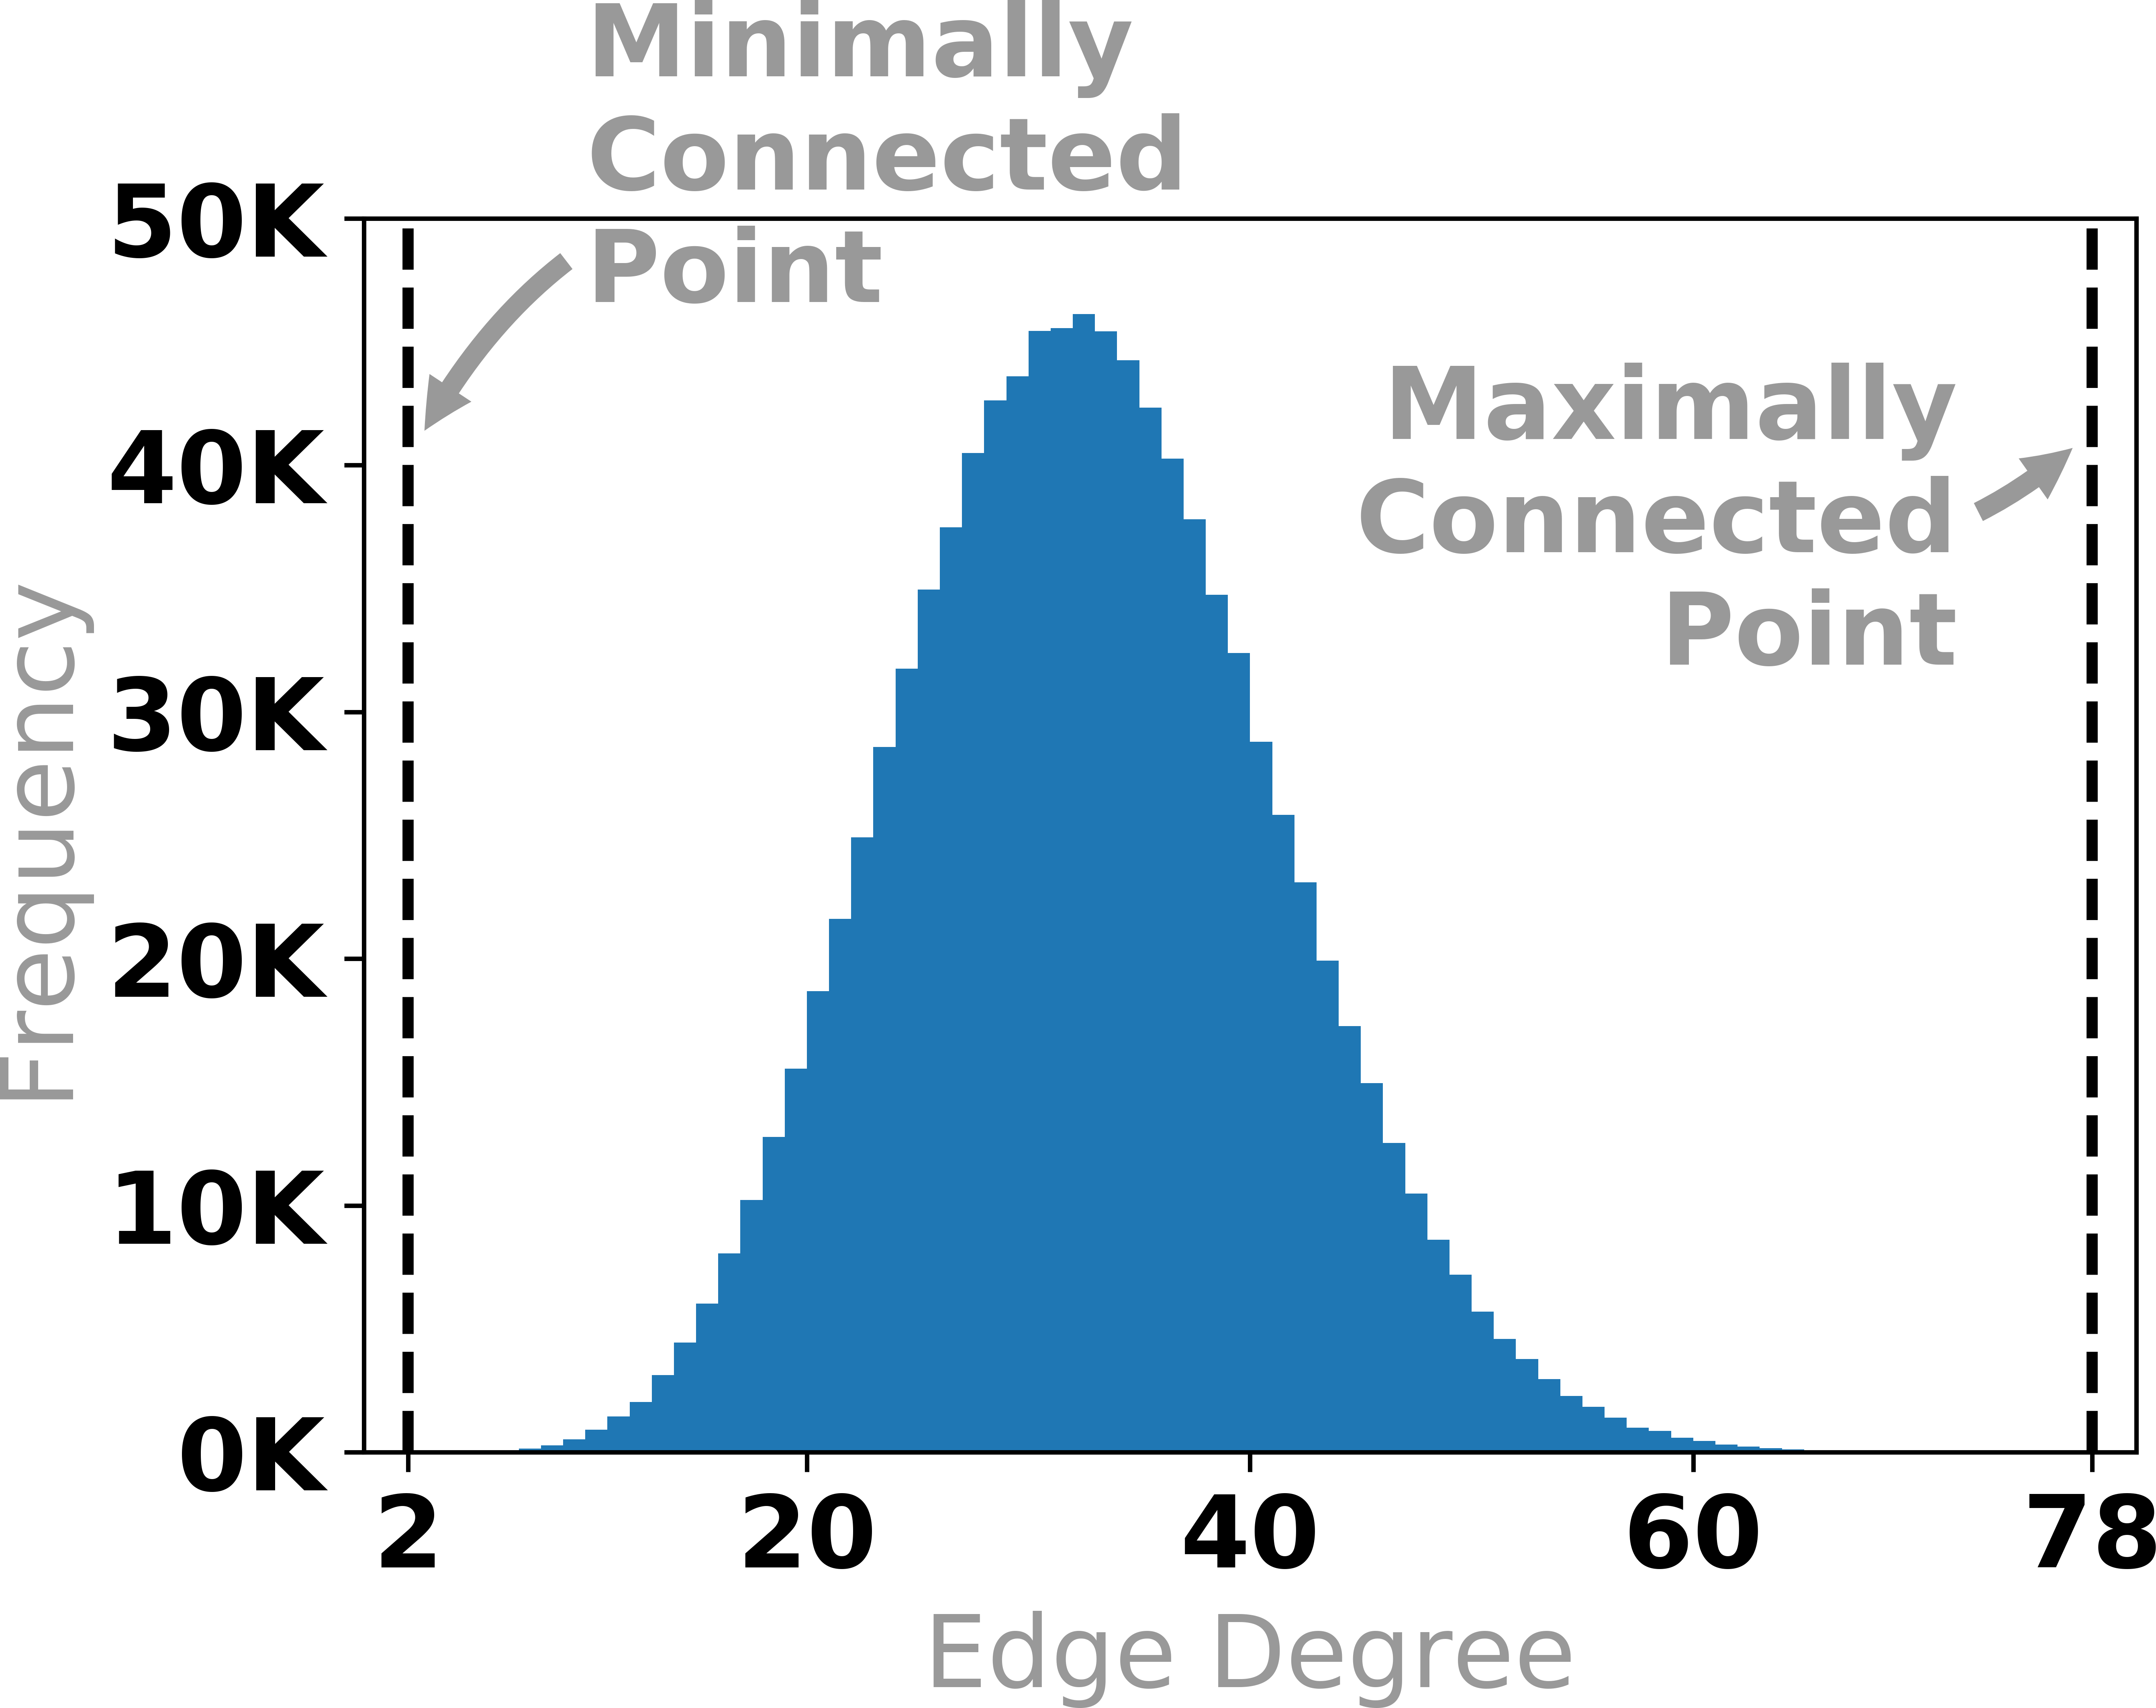
\includegraphics[width=.45\linewidth]{figs/chap7/n-1M_d-5_s-0_k-1000_relaxed_gabriel_histogram.png}
      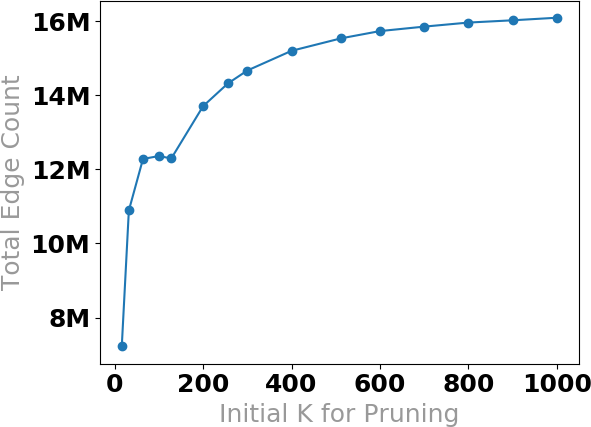
\includegraphics[width=.45\linewidth]{figs/chap7/saturation_1000000_5D.png}
     \caption[Exploration of edge density on five-dimensional Gabriel graph]{
     Left: A histogram of the degree (count of emanating edges) for each point in a symmetric, relaxed Gabriel graph constructed in 5D on a uniformly sampled data with one million points.
     %
     Right: A plot showing the total edges extracted from a symmetric, relaxed Gabriel graph computed on the same dataset as a function of the $k$ used in the initial $k$-nearest neighbor graph.
     %
     Note that the graph begins to level off, meaning adding more $k$ neighbors will not result in any new edges being discovered by the pruned graph.
     }
    \label{fig:graph_degree}
    \vspace{-4mm}
  \end{figure}

The saturation point will vary based on the distribution of the data in the domain.
%
For example, consider a point set that contains $n$ uniformly-spaced samples
on the surface of a ball centered at the origin in $d$-dimensions.
%
If a single point is added at the origin, then all points become connected to
this single point, making the saturation point for this example $k=n$.
%
A demonstration of the $d=2$ case is shown in left image of Figure~\ref{fig:circle_graphs}.

\begin{figure}[b]
    \centering
      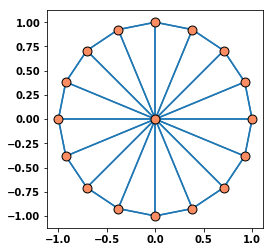
\includegraphics[width=.3\linewidth]{figs/chap7/circle_2.png}
      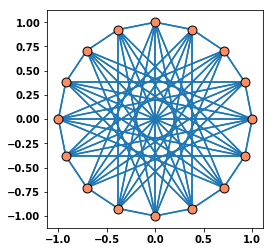
\includegraphics[width=.3\linewidth]{figs/chap7/circle_3.png}
      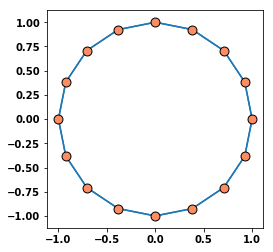
\includegraphics[width=.3\linewidth]{figs/chap7/circle_1.png}
     \caption[Examples of overconnected and underconnected graphs]{Example empty region graphs using $n$ points sampled on the
     surface of a ball. The leftmost image adds a single point at the
     origin, which has a degree of $n$ in the graph. The center image shows
     a relaxed $\beta$-skeleton ($\beta$ < 1) with many crossing edges.
     The leftmost image shows the 2-nearest neighbor graph.
     }
    \label{fig:circle_graphs}
    \vspace{-0.1in}
\end{figure}

However, in other cases it may be beneficial to clip the relaxed empty region graph in order to capture intrinsic structure of the dataset.
%
Going back to our ball example, if we remove the point at the origin, our graph could end up having many crossing edges spanning the interior of the ball, as shown in the center image of Figure~\ref{fig:circle_graphs}.
%
In such a case, using a value of $k$ below the saturation point can better capture the intrinsic structure of the point set, such as the right image that uses $k=2$ to construct the graph.
%
The effects of clipping the empty region and cone graphs with different $k$ values is beyond the scope of this work, although from this initial analysis does present itself as an interesting area requiring further study.

\subsection{Performance Analysis}

In this section, we compare the performance of the existing serial algorithm provided by NGL to our GPU implementation.
%
For this study, both libraries have been modified to accept a precomputed $k$-nearest neighbor graph for pruning, and therefore timing results do not include the computation of the $k$-nearest neighbor graph.
%
We first investigate each library's ability to reconstruct both a strict and relaxed Gabriel graph in dimensions ranging from 2 to 10 dimensions on small (10,000) to moderate ($10^6$) sized problems.
%
We show results for a uniform, random point sampling strategy, but the specific distribution should not significantly impact the running time of either implementation.
%
Additional tests (not included) support this claim, where similar performance is achieved on other strategies such as CVT, LHS, and a normally distributed point set of the same size.
%
For the discrete cases, we use $s=10,000$.
%
The results reported in Figure~\ref{fig:performance} have been averaged over 10 trials, with error bars showing one standard deviation ($1\sigma$).
%
The error bars are hardly perceptible, demonstrating that the deviations in performance for the different algorithms are indeed statistically significant.
%
The top row shows results for the strict Gabriel graph, and the bottom row shows results for the relaxed Gabriel graph.
%
The number of neighbors used in the underlying $k$-nn graph varies commensurate with the dimension, and thus performance is as much a factor of $k$ as of dimensionality in these cases.
%
We see for smaller problems and lower dimensions that both implementations offer competitive speeds, but as the dimensionality and $k$ grow, our implementation is able to offer even more speed-up.
%
Furthermore, the discretized version can add a modest improvement to the GPU algorithm with only minor differences in the resulting graph.

\begin{figure}[htbp]
    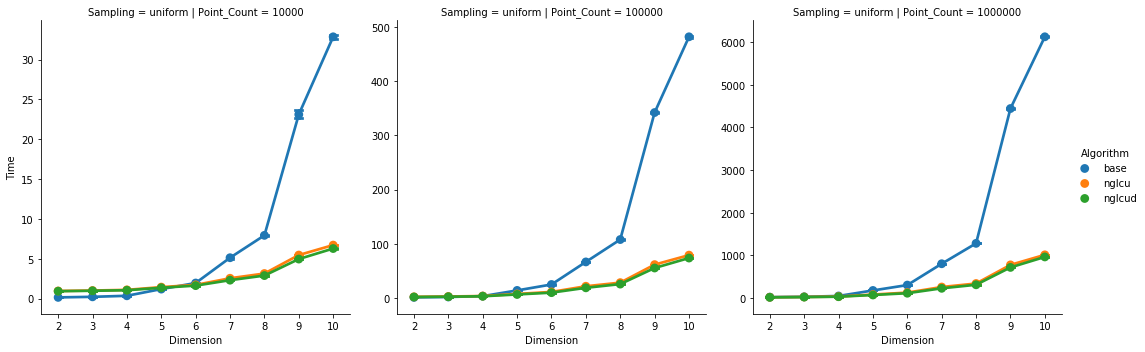
\includegraphics[width=\linewidth]{figs/chap7/strict_performance_d.png}
    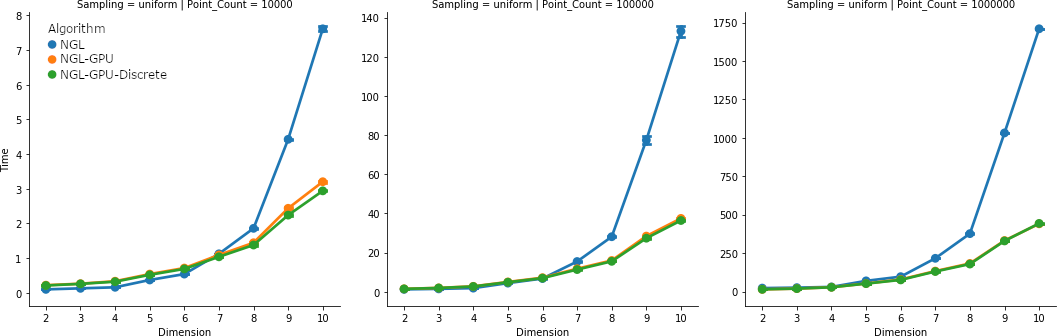
\includegraphics[width=\linewidth]{figs/chap7/relaxed_performance_d.png}
    \caption[Performance of GPU versus serial implementation of Gabriel Graph]{We report the performance of NGL (blue) and two of our GPU
    implementations (standard - orange, and discrete - green) by
    evaluating time as a function of the dimensionality. For the
    dimensionalities listed, we use the following values for $k$ in
    pruning: $d < 5$, $k=100$, $d < 7$, $k=200$, $d < 9$, $k=300$, and
    otherwise $k=500$. From left to right in both rows, the sample sizes
    are 10000, 100000, 1000000.}
    \label{fig:performance}
\end{figure}

\subsection{Two-Dimensional Graph Quality Measures}

Here we evaluate the measures defined in Section~\ref{sec:graph_quality_measures}
on various 2D distributions using a fixed sample size of 200 points.

\begin{figure}[htbp]
  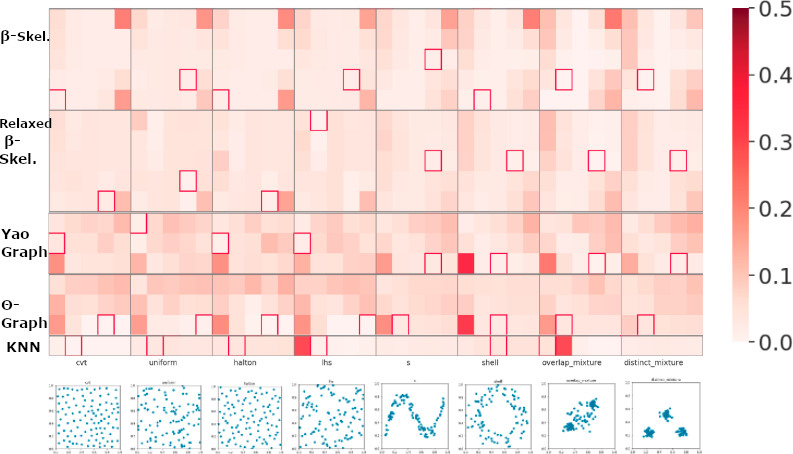
\includegraphics[width=\linewidth]{figs/chap7/Combined5graphs.png}
  \caption[Heatmaps for identifying optimal graph quality]{A graph quality heatmap based on the aggregation of five graph quality measures on five proximity graphs for eight distributions.
  %
  The optimal parameter setting for each graph is highlighted.}
  \label{fig:teaser}
\end{figure}

Figure~\ref{fig:teaser} shows the shows the values of $M_{composite}$ computed over different parameterizations of our 5 graphs, $\beta$-skeleton, relaxed $\beta$-skeleton, Yao graph, $\Theta$-graph, and $k$-nn graph, on 8 distinct distributions of points.
%
Each large gray-outlined box contains multiple subcells denoting the $M_{composite}$ value for various parameter settings, and the optimal setting for each graph is outlined with a red box.
%
Within each box, we evaluate different parameters depending on the graph type.
%
For the empty region graphs, the horizontal axes represent the following $\beta$ values (from left to right): 0.25, 0.5, 1.0, 1.5, and 2.0.
%
The vertical axes represent the following $p$ values (from bottom to top): 0.4, 0.8, 1.0, 2.0, and 4.0.
%
For the cone graphs, the horizontal axes represent the following $c$ cone counts (from left to right): 1, 2, 3, 4, and 5.
%
The vertical axes represent the following $m$ points per cone counts (from bottom to top): 1, 2, and 3.
%
For the $k$-nn graph, there is only one parameter $k$, and we show the following values (from left to right): 1, 2, 3, 4, and 5.
%
When evaluating the heatmap, lower values are better for our quality measure.
%
According to the quality measure shown in Figure~\ref{fig:teaser}, there are no universal optimal parameters for different distributions and sample sizes, although we do see some trends.
%
For instance, with the 4 non-space-filling distributions on the right that somehow have an intrinsic shape that is different from their embedding domain, the relaxed $\beta$-skeleton tends to do well with the setting $\beta=1.5$ and $p=2$, whereas the Yao and $\Theta$ graphs tend to favor $m=1$ for those cases.
%
The strict $\beta$-skeleton seems to favor lower $p$ values for all cases.

In Figure~\ref{fig:graph_quality}, we attempt to directly compare the optimal graph performance for the composite graph measure for each of the eight distributions considered.
%
Note, we explore a more thorough search space than the values presented in Figure~\ref{fig:teaser}.
%

%
We find that under the most generic setting of our composite measure, the strict $\beta$-skeleton performs best on average and the relaxed $\beta$ graph is consistently the worst performing.
%
Examples of each distribution with their $\alpha$-shapes are shown with the optimal graphs from each category overlaid on top in Figures~\ref{fig:bs_quality}-~\ref{fig:theta_quality}.
%
From these figures, we can see that when the topology is not simply connected, the relaxed $\beta$-skeleton is unable to recover the shape well and despite using a larger empty region, still tends to overconnect the domain.
%
This study suggests that when operating on non-simply-connected domains, the difference between the strict and relaxed $\beta$-skeleton is indeed significant.
%
Furthermore, the Yao graph represents a good compromise between quality and efficiency for most cases, given that it does not suffer from the memory overhead seen in the strict $\beta$-skeleton and thus scales better with dimension $k$ and the size of the data.
%
Additionally, in practice the Yao graph is slightly faster than even the relaxed $\beta$-skeleton.
%
Tuning the parameters for the Yao and $\Theta$ graphs for high-dimensional data is arguably more challenging than for the $\beta$ skeletons where the traditional Gabriel graph ($\beta=1, p=2$) gives a good overall performance for most cases.

\begin{figure}[htbp]
    \centering
    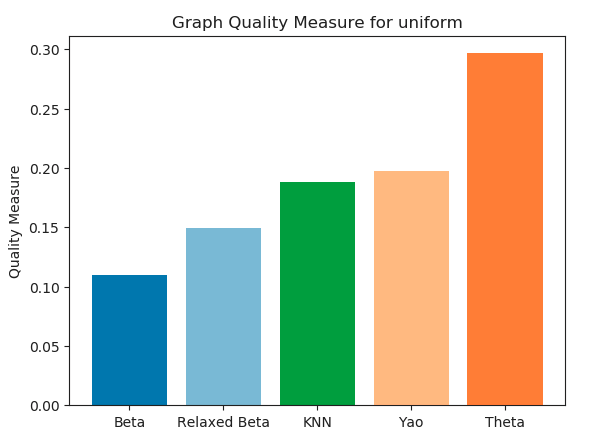
\includegraphics[width=0.45\linewidth]{figs/chap7/uniform_quality.png}
    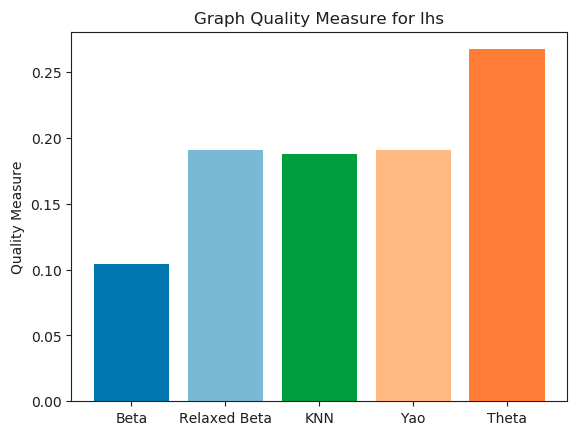
\includegraphics[width=0.45\linewidth]{figs/chap7/lhs_quality.png}
    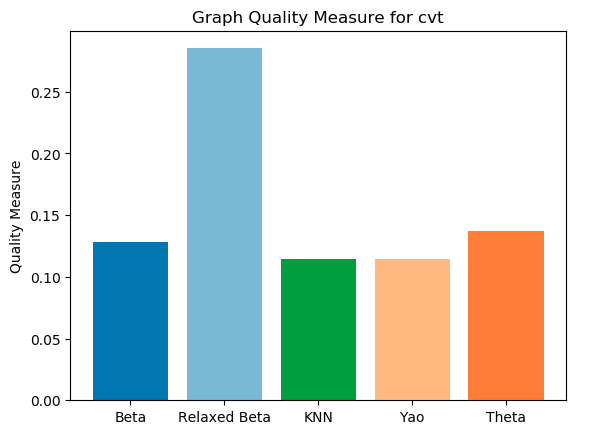
\includegraphics[width=0.45\linewidth]{figs/chap7/cvt_quality.png}
    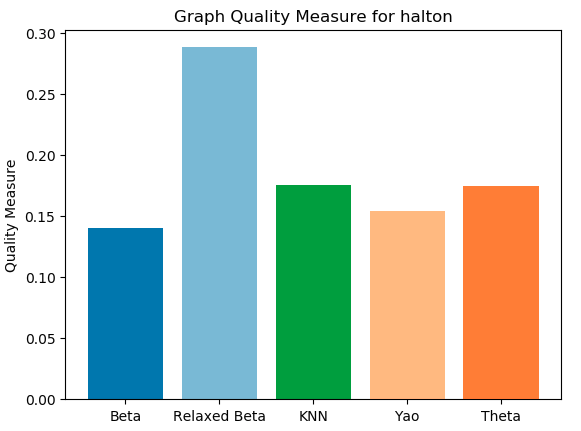
\includegraphics[width=0.45\linewidth]{figs/chap7/halton_quality.png}
    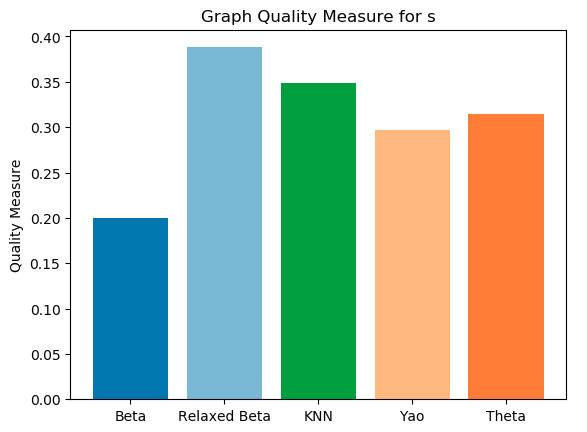
\includegraphics[width=0.45\linewidth]{figs/chap7/s_quality.png}
    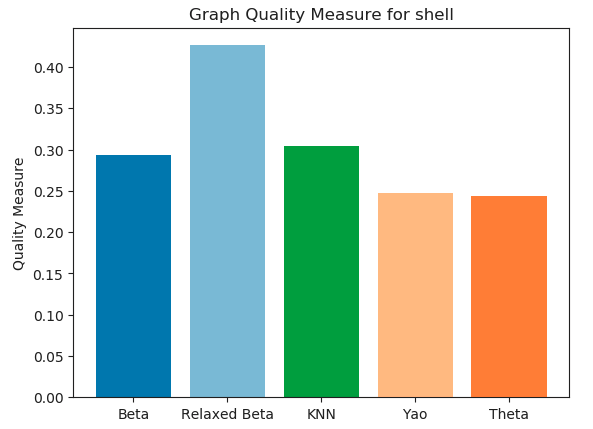
\includegraphics[width=0.45\linewidth]{figs/chap7/shell_quality.png}
    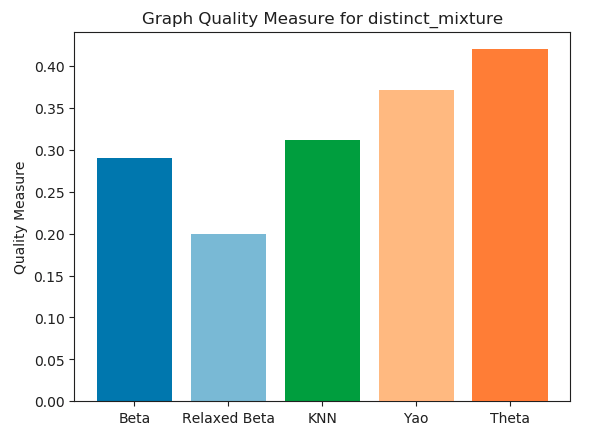
\includegraphics[width=0.45\linewidth]{figs/chap7/distinct_quality.png}
    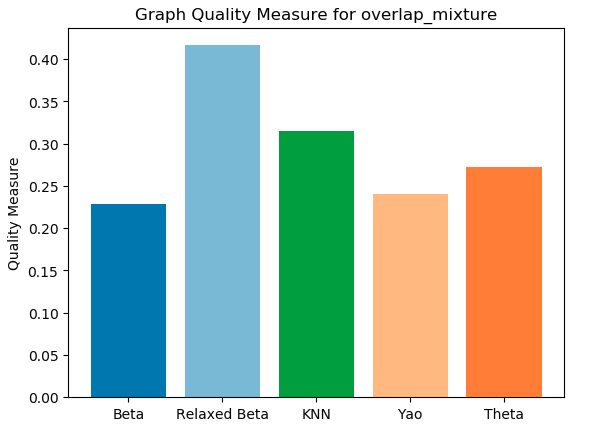
\includegraphics[width=0.45\linewidth]{figs/chap7/overlap_quality.png}
    \caption[Two-dimensional optimal graph quality results]{Analysis of five graphs using our graph quality measures.
    %
    Once an optimal setting is decided for each distribution, we compare it with the optimal composite quality measures of the other graphs.
    %
    The figures rows are described from left to right below.
    %
    Top row: a uniform distribution and an LHS design.
    %
    Second row: a CVT design and a Halton sequence.
    %
    Third row: a sinusoidal shaped manifold and an annulus.
    %
    Bottom row: a mixture of three distinct normal distributions with low probability of overlap, and a mixture with the same centers but with significant overlap.}
    \label{fig:graph_quality}
\end{figure}

\begin{figure}[htbp]
    \centering
    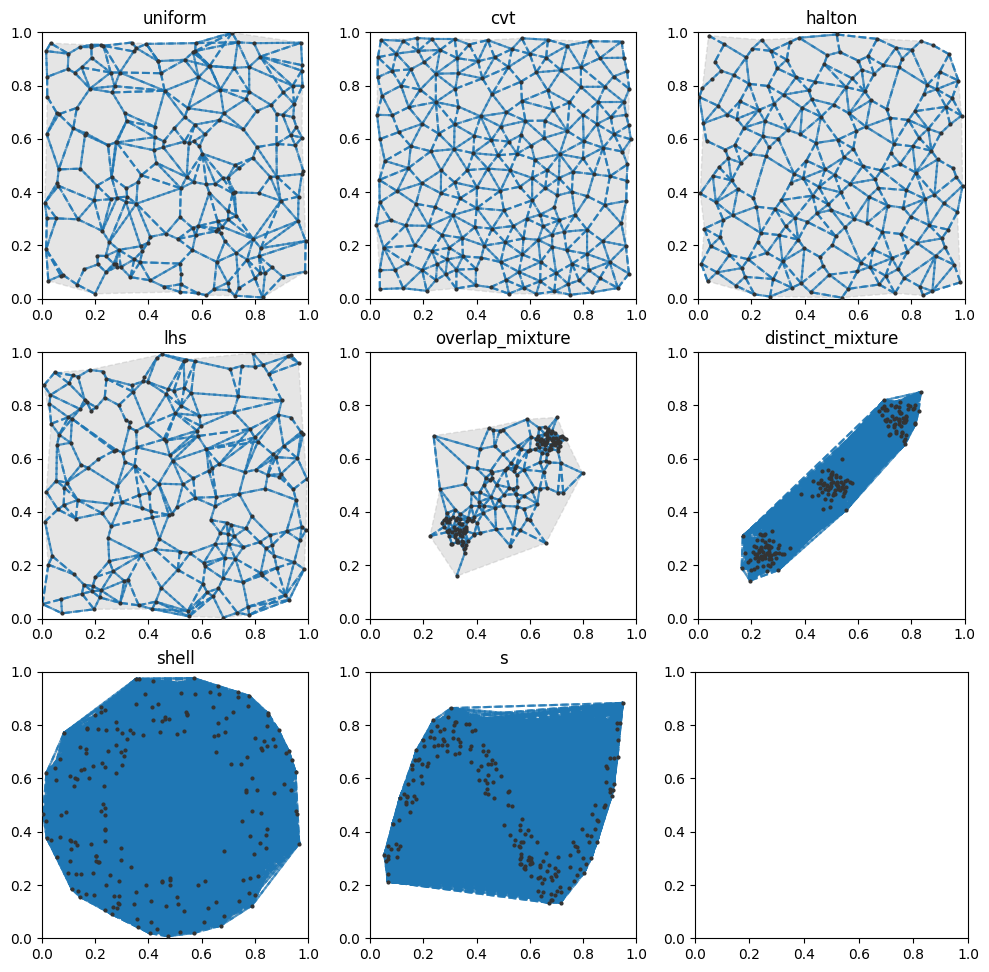
\includegraphics[width=\linewidth]{figs/chap7/bs_quality.png}
    \caption[Optimal strict $\beta$-skeletons for various two-dimensional distributions]{Examples of the best performing strict $\beta$-skeleton are shown for each distribution under consideration.}
    \label{fig:bs_quality}
\end{figure}

\begin{figure}[htbp]
    \centering
    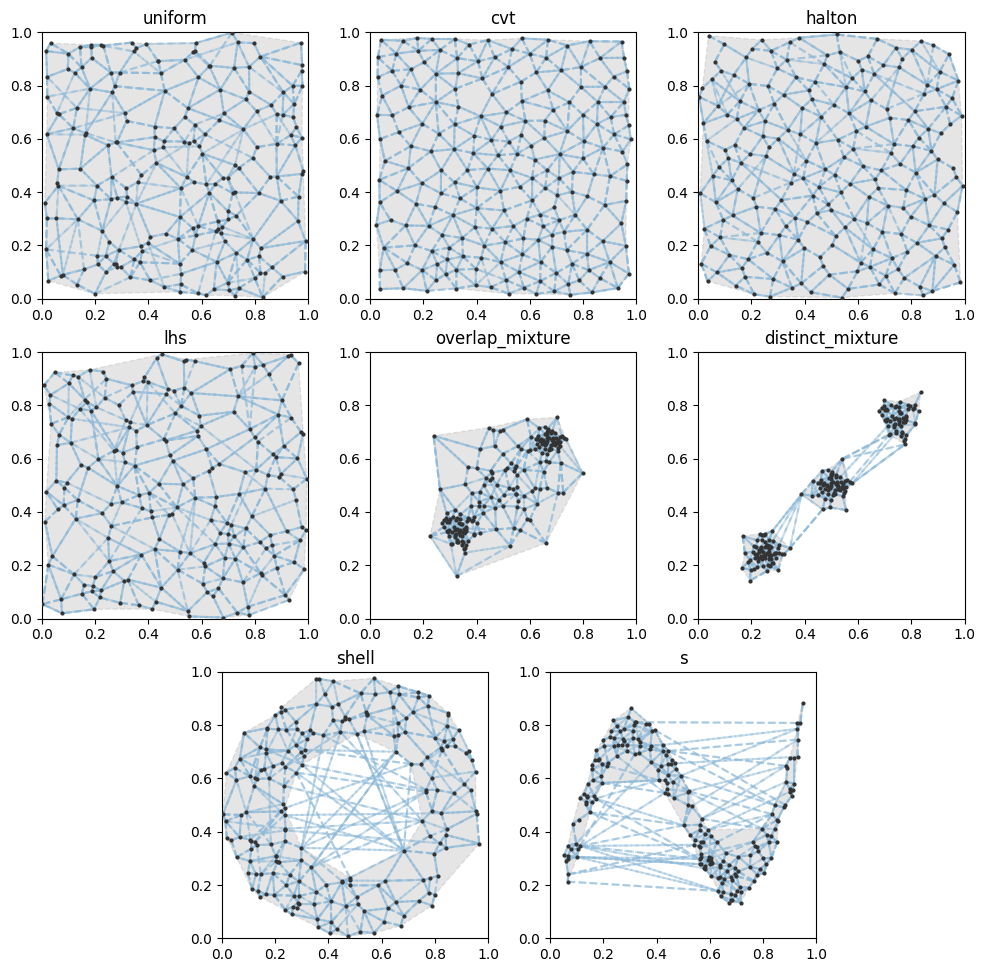
\includegraphics[width=\linewidth]{figs/chap7/rbs_quality.png}
    \caption[Optimal relaxed $\beta$-skeletons for various two-dimensional distributions]{Examples of the best performing relaxed $\beta$-skeleton are shown for each distribution under consideration.}
    \label{fig:rbs_quality}
\end{figure}

\begin{figure}[htbp]
    \centering
    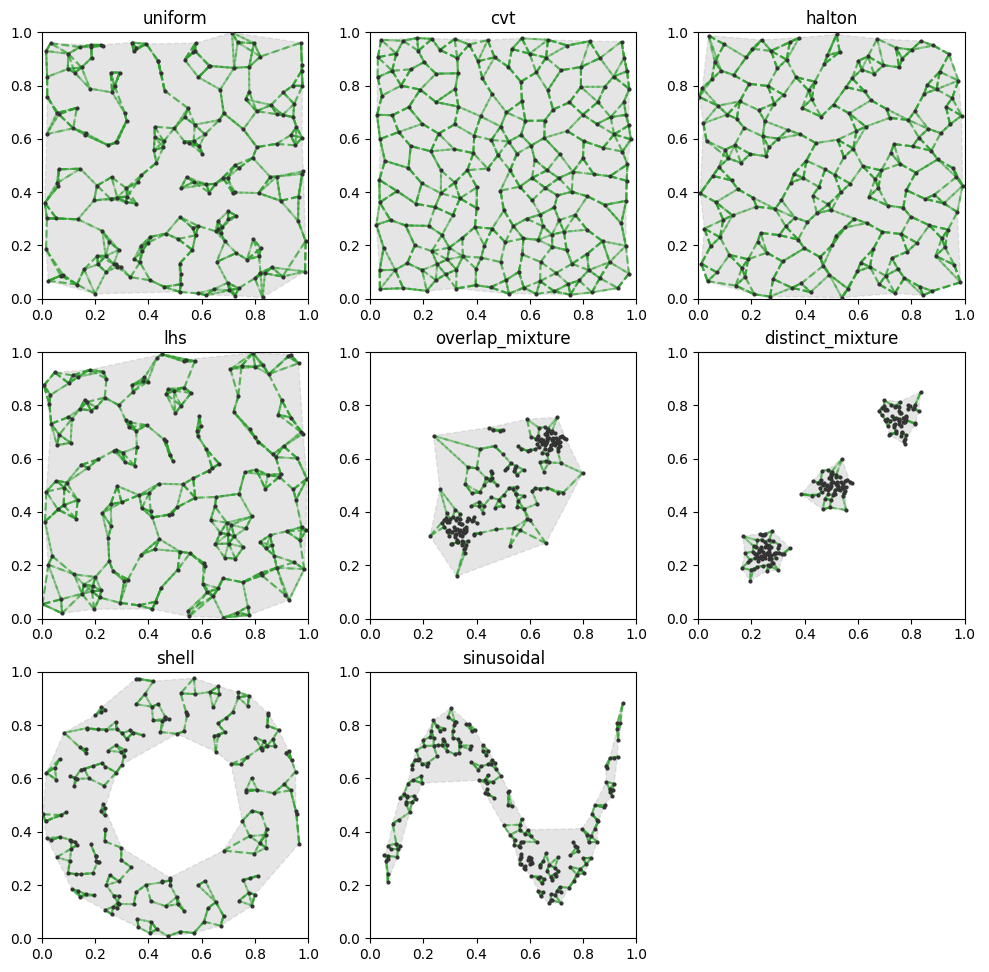
\includegraphics[width=\linewidth]{figs/chap7/k_quality.png}
    \caption[Optimal $k$-nn graphs for various two-dimensional distributions]{Examples of the best performing $k$-nearest neighbor graphs are shown for each distribution under consideration.}
    \label{fig:k_quality}
\end{figure}
\begin{figure}[htbp]
    \centering
    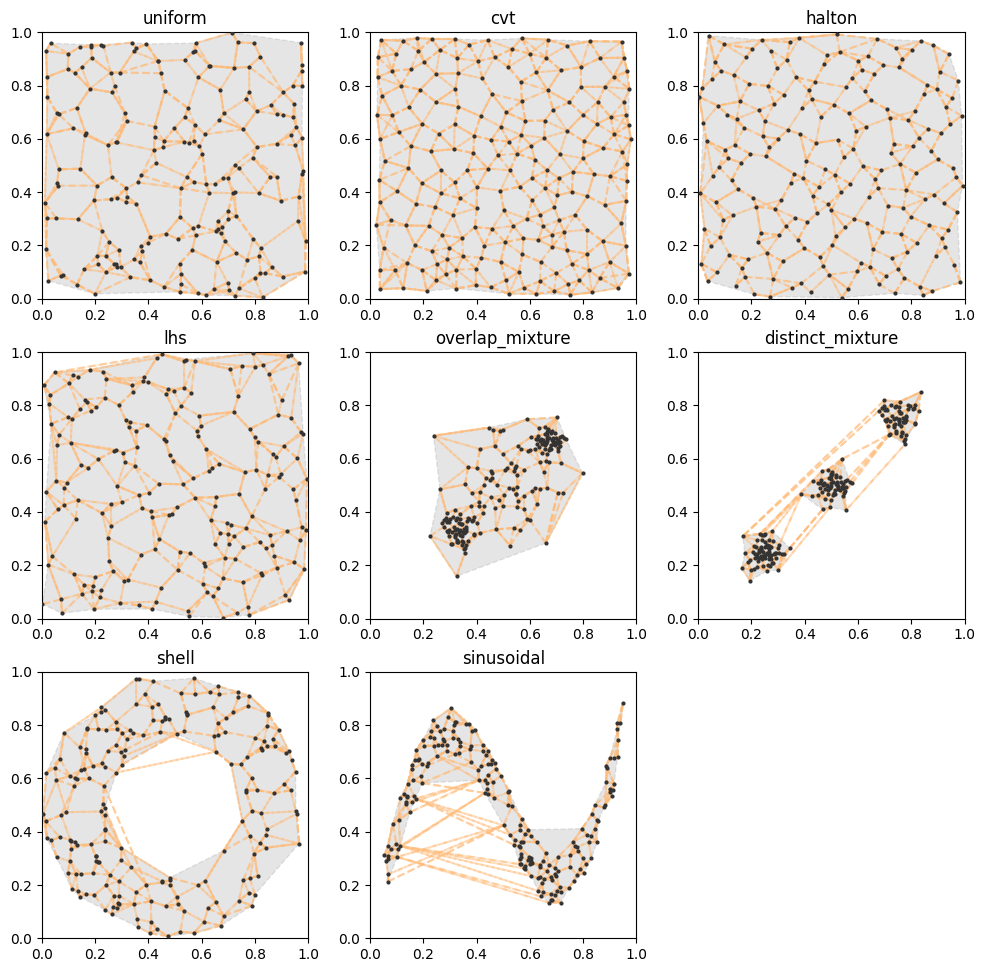
\includegraphics[width=\linewidth]{figs/chap7/yao_quality.png}
    \caption[Optimal Yao graphs for various two-dimensional distributions]{Examples of the best performing Yao graphs are shown for each distribution under consideration.}
    \label{fig:yao_quality}
\end{figure}

\begin{figure}[htbp]
    \centering
    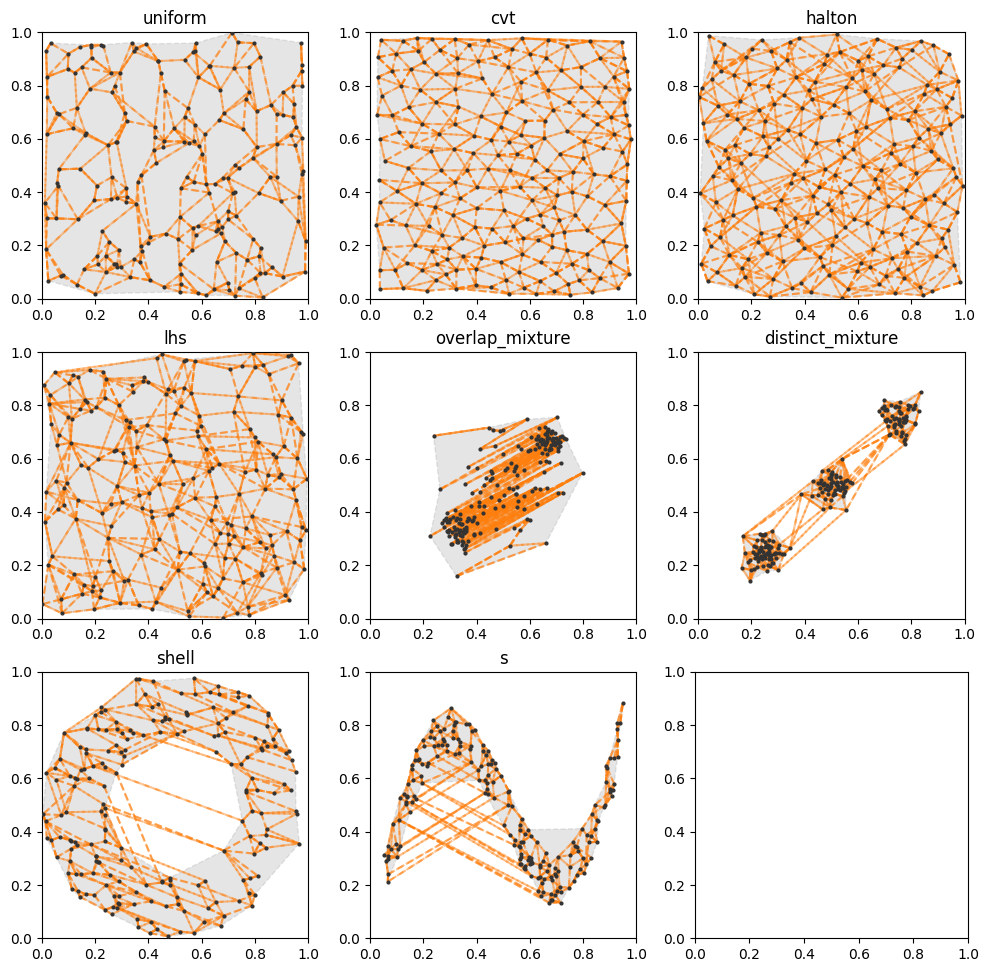
\includegraphics[width=\linewidth]{figs/chap7/theta_quality.png}
    \caption[Optimal $\Theta$-graphs for various two-dimensional distributions]{Examples of the best performing $\Theta$-graph are shown for each distribution under consideration.}
    \label{fig:theta_quality}
\end{figure}

\begin{table}[htbp]
    \scriptsize
    \centering
    \begin{tabular}{| l || c | c | c | c | c |}
    \hline
    \textbf{Distribution}  & \textbf{Strict $\beta$-Skeleton} & \textbf{Relaxed $\beta$-Skeleton} & \textbf{$k$-NN Graph} & \textbf{Yao Graph} & \textbf{$\Theta$ Graph} \\
    \hline
    \textbf{Uniform} & $\beta=0.25, p=0.8$ & $\beta=1, p=2$  & $k=4$ & $c=3, m=1$ & $c=3, m=1$\\
    \textbf{CVT} & $\beta=1, p=2$ & $\beta=1, p=4$  & $k=4$ & $c=1, m=4$ & $c=4, m=1$\\
    \textbf{Halton} & $\beta=1, p=2$ & $\beta=1, p=2$  & $k=4$ & $c=3, m=1$ & $c=4, m=1$\\
    \textbf{LHS} & $\beta=0.25, p=0.8$ & $\beta=1, p=2$  & $k=4$ & $c=3, m=1$ & $c=4, m=1$\\
    \textbf{Overlapping Mixture} & $\beta=0.5, p=0.8$ & $\beta=1, p=2$  & $k=3$ & $c=3, m=1$ & $c=4, m=1$\\
    \textbf{Distinct Mixture} & $\beta=0.25, p=0.8$ & $\beta=1, p=2$  & $k=3$ & $c=3, m=1$ & $c=4, m=1$\\
    \textbf{Shell} & $\beta=0.25, p=0.8$ & $\beta=1, p=2$  & $k=3$ & $c=3, m=1$ & $c=3, m=1$\\
    \textbf{Sinusoidal} & $\beta=1, p=2$ & $\beta=1, p=2$  & $k=3$ & $c=3, m=1$ & $c=3, m=1$\\
    \hline
    \end{tabular}
    \caption[Optimal graph parameters used in Figures~\ref{fig:graph_quality}-~\ref{fig:theta_quality}]{Optimal parameter settings used for each test distribution shown in Figures~\ref{fig:graph_quality}-~\ref{fig:theta_quality}.}
    \label{tab:optimal_settings_quality}
\end{table}

\subsection{Topological Accuracy and Stability}

Empty region graphs have been shown to be useful for providing the necessary structure for approximating topological structures on multidimensional point cloud data~\cite{BremerMaljovecSaha2014,CorreaLindstrom2011,LiebmannWeberScheuermann2018,MaljovecLiuWang2016,MaljovecWangRosen2016}.
%
In this section, we evaluate the ability of our three families of graphs to extract the topology of different synthetic functions in varying dimensions using several different point samples.
%
Specifically, we look at approximating the Morse complex using the algorithm from Gerber et al.~\cite{GerberBremerPascucci2010} and computing the persistence hierarchy to understand not only the accuracy but also the stability of the correct result.
%
We compare these results to a ground-truth acquired through either numerical methods or by exploiting the simple geometry of the test functions Morse complex.
%
To compare our approximated results to the ground-truth, we use persistence simplification~\cite{EdelsbrunnerLetscherZomorodian2002,EdelsbrunnerHarer2008} to denoise our approximation to the correct number of manifolds.
%
We then compute the normalized variation of information~\cite{VinhEppsBailey2010} to compute the level of correspondence between the two partitions.
%
This metric is borrowed from the field of information theory where it is commonly used to evaluate clustering results.
%
It is a true metric, and the normalized version has the added property of existing on the range of [0,1], where 0 means perfect agreement.
%
Lastly, we want to evaluate not only the accuracy of the segmentation, but arguably more importantly, the stability of the segmentation.
%
For this, we again rely on the persistence hierarchy to compute the \textit{lifespan} of the correct partition.
%
We define the lifespan as the range of persistence values over which the Morse complex retains the correct segmentation.
%
Higher values are preferred because they indicate that the graph is able to report the ``correct'' partition over a larger range of persistence values.
%
However, the stability is useful only if we validate that the NVI is low enough to assume that the partitions are well-aligned.

For testing, we utilize a few highly controllable synthetic test functions described below.
%
Each class of functions allows varying levels of topological complexity and can be generalized to any dimension.
%
The functional form of the chosen class of functions is sufficiently general to generate a wide variety of response surfaces.
%
In addition, these functions are parameterized by the location of centers as well as the degree of smoothness.
%
The number of centers also defines the number of maxima present and thus controls the number of features present in the generated dataset.
%
The first of these functions is the diagonal test function, where we take the tensor product of a sine curve aligned with the main diagonal of the $d$-dimension space and a Gaussian kernel falling off in the hyperplane orthogonal to the main diagonal.
%
By restricting the function to a fixed domain, we can readily set the number of maxima/minima occurring in the sample space by varying the period of the sine curve.
%
In closed form, this function is expressed as,
%
\begin{eqnarray*}
    f(\mathbf{x}) = \frac{1}{2}\sin\left(\pi\left(\frac{1}{2} + \left((m+1)
      \bmod{2}\right) + \frac{m\left(\sum_{i=1}^{d}x_i\right)}{d}\right)\right)
    \\
     \times e^{\left(\left(\sum_{i=1}^{d}x_i^2 -\frac{\left(\sum_{i=1}^{d}
      x_i\right)^2}{d}\right)\left(\frac{\log(0.001)}{\sqrt{d}}\right)\right)},
\end{eqnarray*}
%
where each $x_i$ is in the range $[-1,1]$, $d$ denotes dimension and $m$ is the number of maxima along the main diagonal.

The \emph{Distance Field (DF)} function in closed form is expressed as $f(\mathbf{x}) = -\bigl(\sum_i \langle\mathbf{x}-\mathbf{c_i},A_i(\mathbf{x}-\mathbf{c_i})\rangle^{p/2}\bigr)^{1/p}$, where the parameter $p < 0$ allows tuning the smoothness of this approximation to a nondifferentiable distance field ($p = -\infty$ gives a true distance field).
%
$A_i$ is a $d \times d$ randomly generated covariance matrix associated to the $i^{th}$ center, and $\mathbf{c_i}$ is the vector defining the location of the $i^{th}$ center.
%
The convenience of these functions is that the locations of the true maxima are known and can be added to our sample sets.
%
We can then measure an approximation's ability to correctly detect these features.
%
Figure \ref{fig:datasets} visually depicts 2D versions of the test functions where we use two different values for the .
%
The blue regions denote regions of maxima whereas the orange/brown regions denote regions of minima.
In addition, blue dots represent local maxima, white dots represent saddle points, red dots denote local minima, and the thick lines separate the cells of the Morse complex of the function, $f$.

\begin{figure}[htbp]
    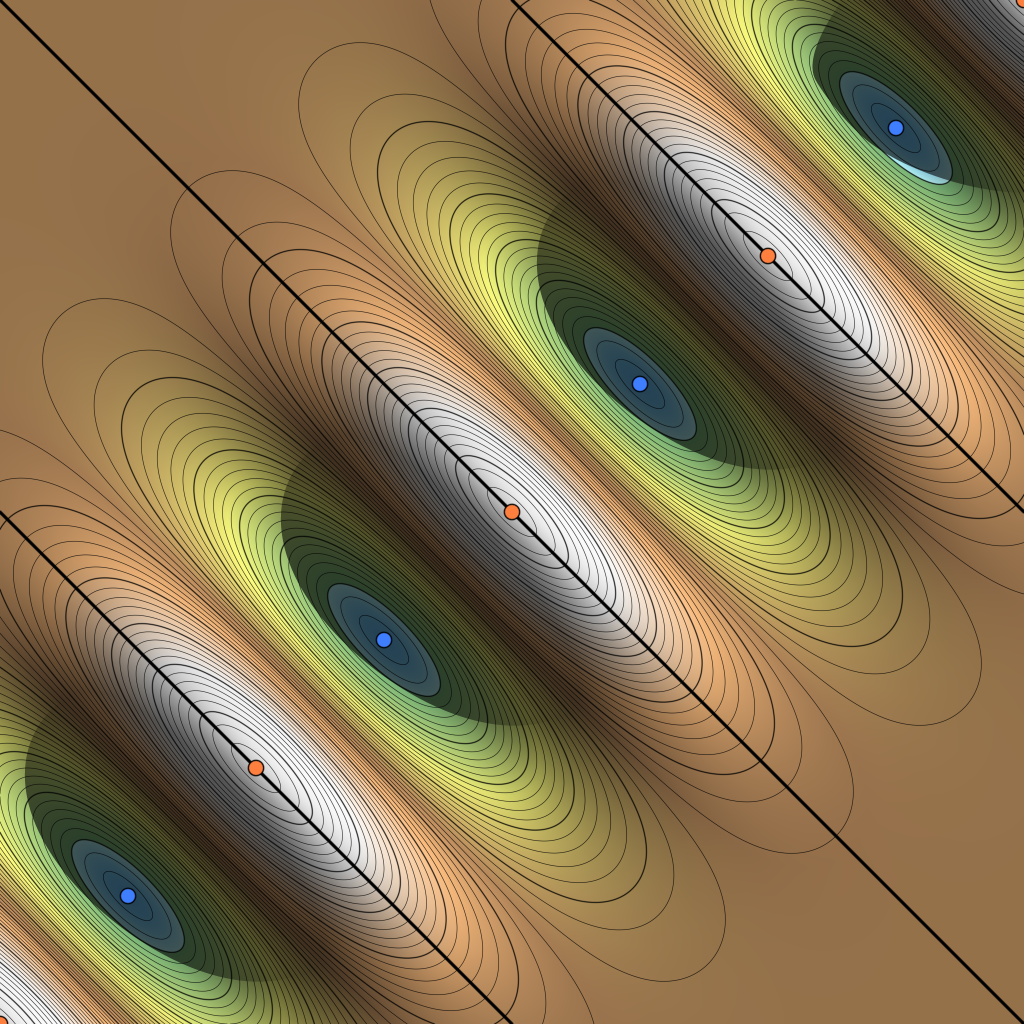
\includegraphics[width=0.32\textwidth]{figs/chap7/diag4.png}
    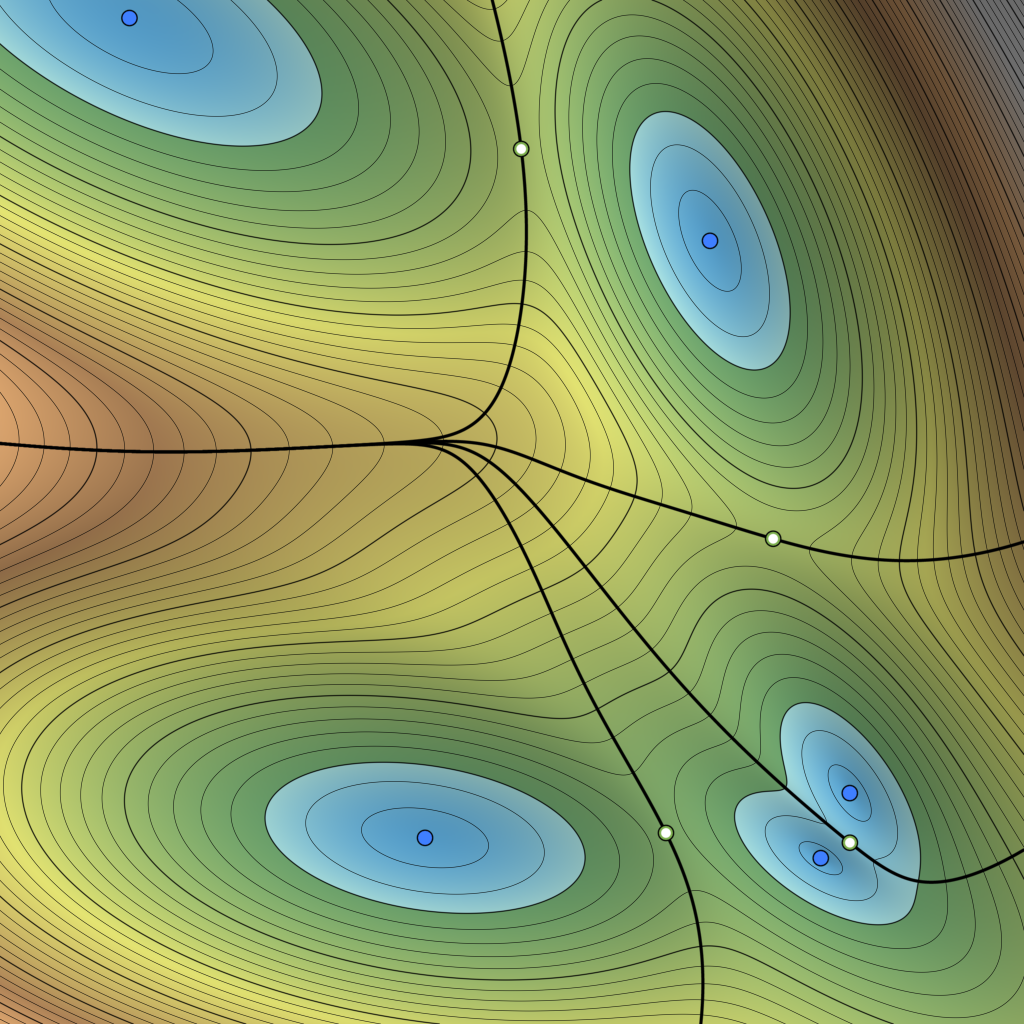
\includegraphics[width=0.32\textwidth]{figs/chap7/df5.png}
    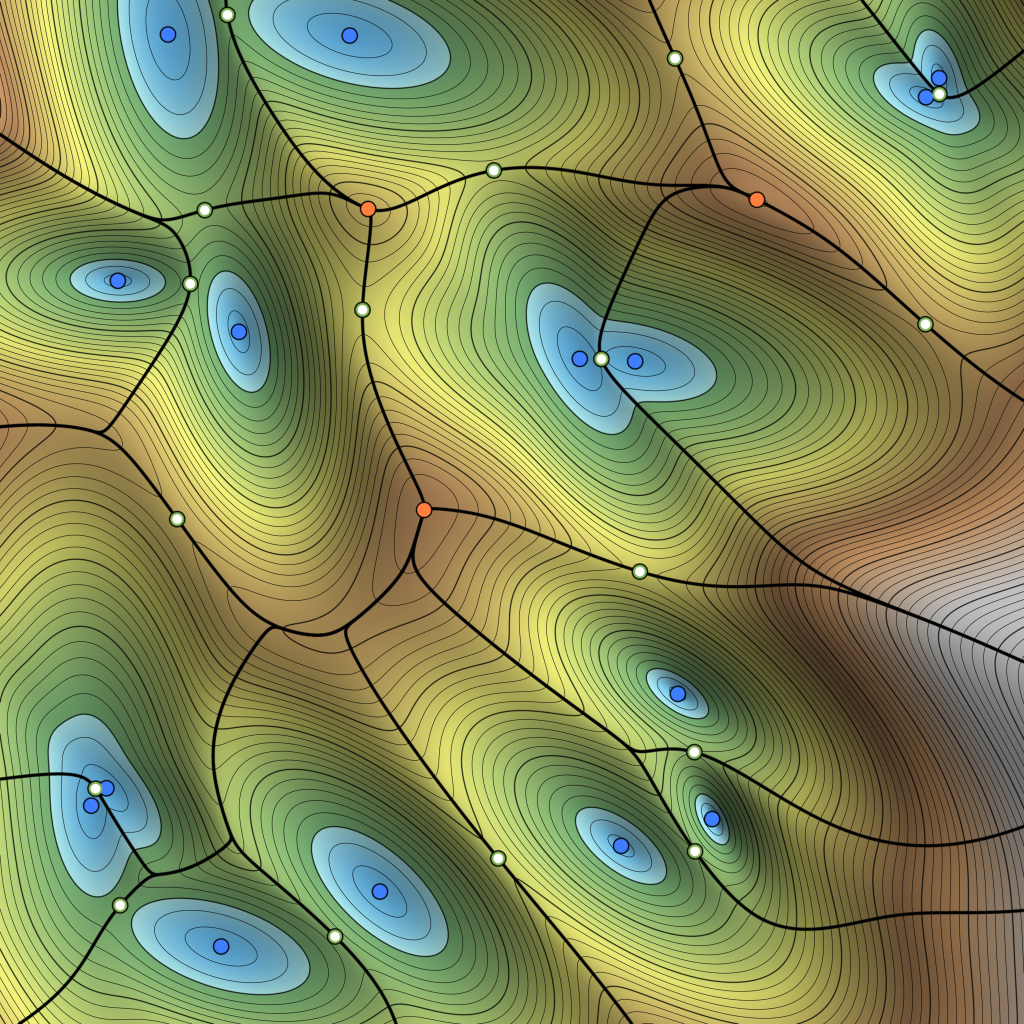
\includegraphics[width=0.32\textwidth]{figs/chap7/df15.png}
    \caption[Two-dimensional test functions for topological stability analysis]{Visual representations of our three test functions in two dimensions.}
    \label{fig:datasets}
\end{figure}

To compute the ground-truth for the diagonal dataset, we can separate the four true segments in closed form by defining hyperplanes through each of three uniformly spaced minima and orthogonal to the main diagonal.
%
For more generic examples, we can formulate a ground-truth labeling of the input data by employing a fourth-order Runge-Kutta scheme to trace the gradient from any point in the domain to its associated maximum.

As with the quality measures, we first evaluate each graph family in isolation and determine the optimal settings for each example function and dimensionality before summarizing and comparing results between the different graphs.
%
Here, we optimally tune each graph for the most consistently high stable persistence.
%
The summarized results are presented in Figure~\ref{fig:graph_topo} for three examples in 4D and 5D.
%
The NVI plots are used mostly for validation to indicate that the partitions we are considering as stable line up consistently with the underlying ground-truth.

The results of this study seem to indicate that the $\Theta$-graph is unable to converge on the correct topology for any of our examples, and whereas the others report similar NVI behavior, the optimal Yao graph is able to achieve this level of fidelity for the largest amount of persistence consistently across the three examples.
%
We report the optimal parameter settings for the examples shown in Figure~\ref{fig:graph_topo} in Table~\ref{tab:optimal_settings}.

\begin{figure}[htbp]
    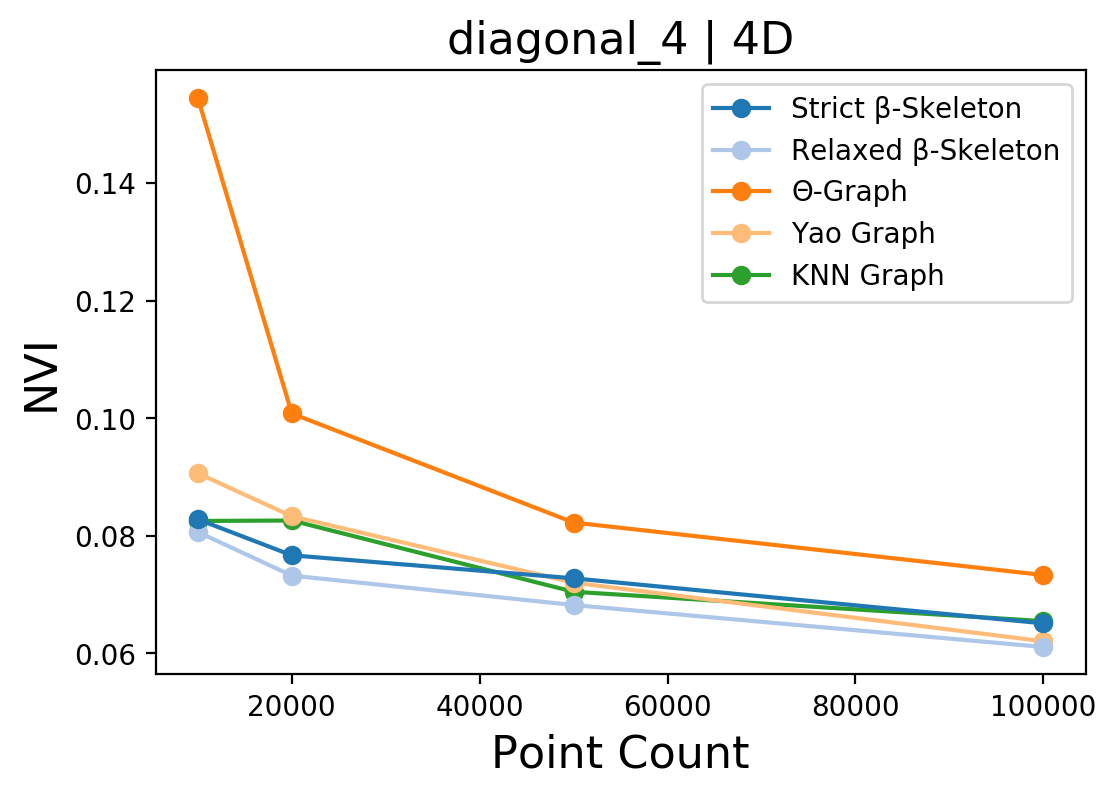
\includegraphics[width=0.48\linewidth]{figs/chap7/diagonal_4_nvi.png}
    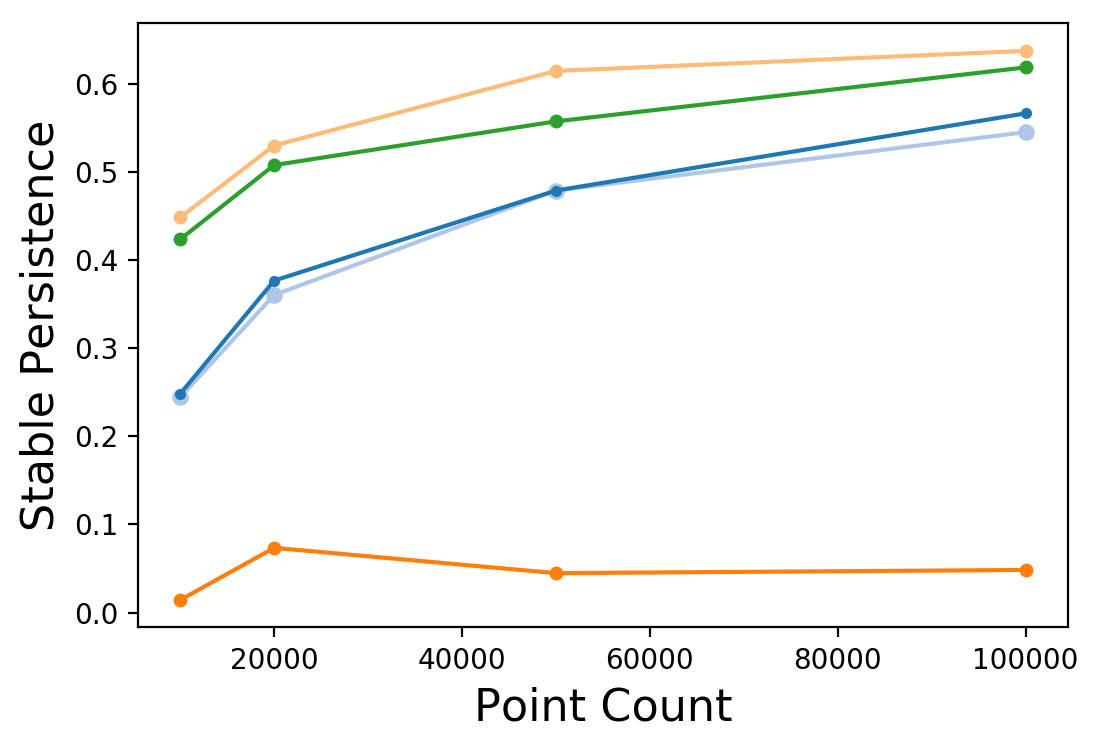
\includegraphics[width=0.48\linewidth]{figs/chap7/diagonal_4_stability.png}
    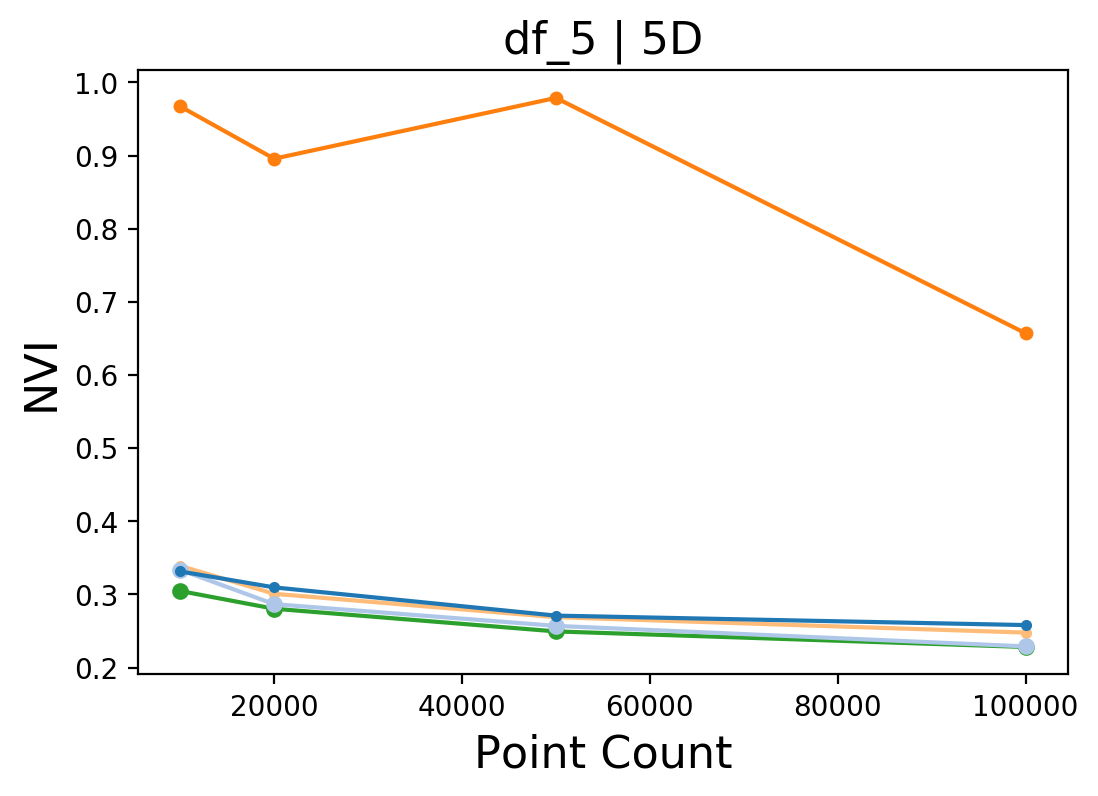
\includegraphics[width=0.48\linewidth]{figs/chap7/df_5_5D_nvi.png}
    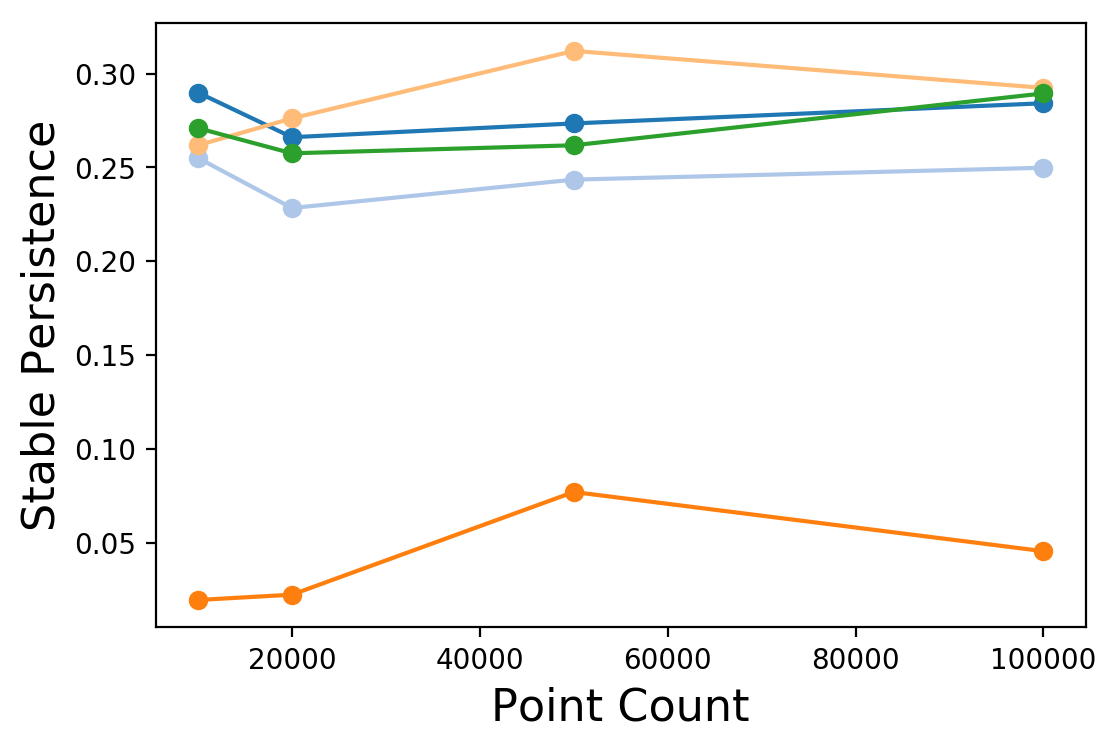
\includegraphics[width=0.48\linewidth]{figs/chap7/df_5_5D.png}
    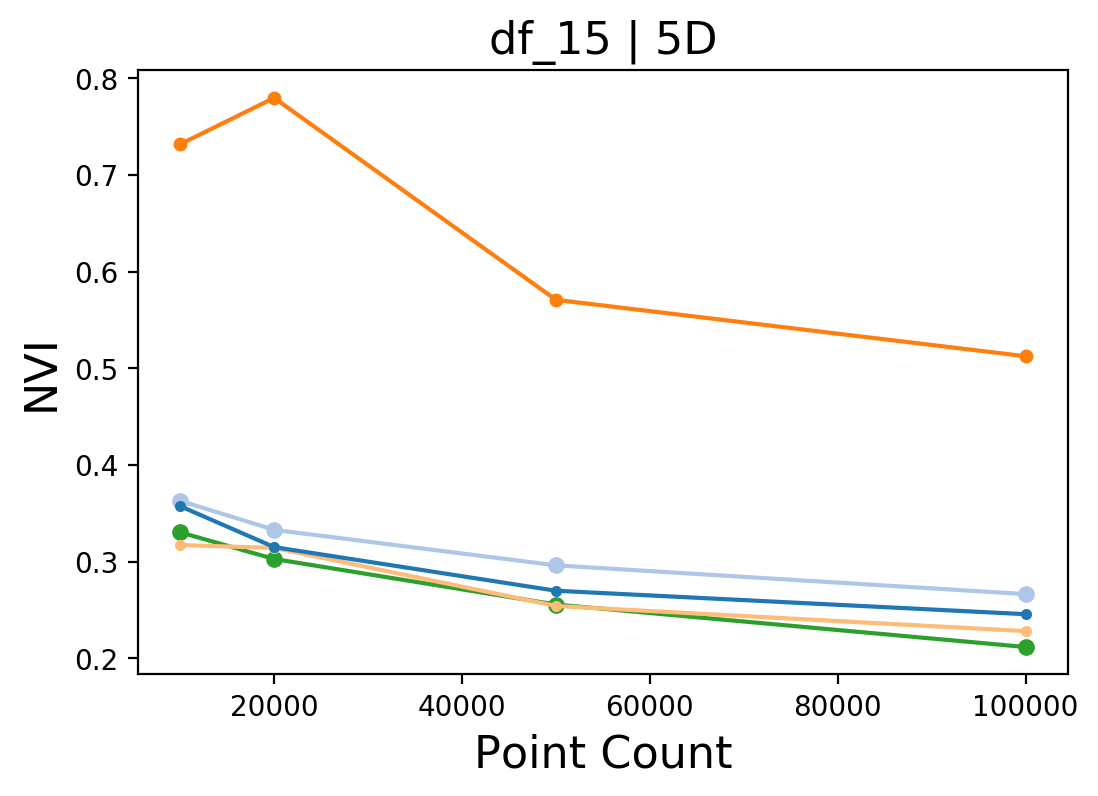
\includegraphics[width=0.48\linewidth]{figs/chap7/df_15_5D_nvi.png}
    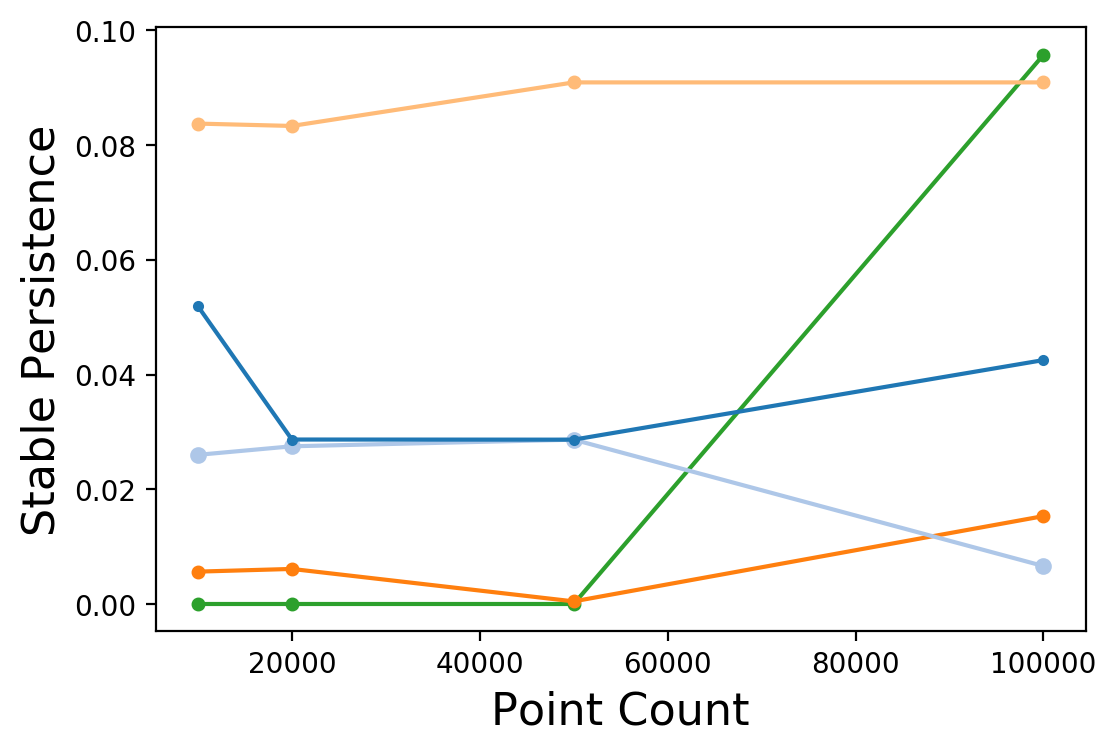
\includegraphics[width=0.48\linewidth]{figs/chap7/df_15_5D.png}
    \caption[Analysis of graphs for topological stability]{Analysis of five graphs under the topological setting for various test functions in varying dimensions using various sample sizes.
    Left: The NVI of the best-in-class for each graph.
    %
    Right: Along with NVI we report the persistence lifespan that each graph is able to maintain the correct partition.
    Top Row: Diagonal test function in four dimensions.
    Middle Row: A distance field function with five maxima in five dimensions.
    Bottom Row: A distance field function with 15 maxima in five dimensions.}
    \label{fig:graph_topo}
\end{figure}

\begin{table}[htbp]
    \scriptsize
    \centering
    \begin{tabular}{| l | c | c | c |}
    \hline
    \textbf{Graph}  & \textbf{4D Diagonal with 4 maxima} & \textbf{5D DF with 5 maxima} & \textbf{5D DF with 15 maxima} \\
    \hline
    Strict $\beta$-Skeleton & $\beta=0.5, p=2$ & $\beta=1, p=2$  & $\beta=1, p=4$ \\
    Relaxed $\beta$-Skeleton & $\beta=0.5, p=4$ & $\beta=1, p=1$  & $\beta=1.5, p=2$ \\
    $k$-Nearest Neighbor Graph & $k=128$ & $k=64$  & $k=64$ \\
    Yao Graph & $c=32, m=2$ & $c=10, m=3$  & $c=32, m=1$ \\
    $\Theta$ Graph & $c=24, m=2$ & $c=25, m=1$  & $c=20, m=2$ \\
    \hline
    \end{tabular}
    \caption[Optimal graph parameters used in Figure~\ref{fig:graph_topo}]{Optimal parameter settings used for each test function shown in Figure~\ref{fig:graph_topo}.}
    \label{tab:optimal_settings}
\end{table}

\subsection{SVM Classification Enhancement}

Various studies have shown that utilizing proximity graphs can effectively reduce the amount of data needed to train a classifier with little to no impact on the trained model's accuracy~\cite{BhattacharyaPoulsenToussaint1981,GotoIshidaUchida2015,Toussaint2005,ToussaintBerzan2012,ZhangKing2002a,ZhangKing2002b}.
%
Here, we attempt to replicate some of these studies by preprocessing a dataset with our various graphs and evaluate both their ability to reduce the training size and the accuracy they are able to maintain.
%
The difference in our study is that we compare across empty region graphs, cone graphs, and $k$-nn graphs, and we also consider the various parameter settings of each.
%
We perform this study in a regime similar to that of Zhang and King~\cite{ZhangKing2002a,ZhangKing2002b}.
%
Under this setting, we use an SVM (see Section~\ref{sec:svm} for details) to train our data and use the subset of edges that lie on the decision boundary (the endpoints of an edge belong to separate classes) to train the SVM.
%
This idea takes advantage of the fact that the SVM is made up of \textit{support vectors} that describe the boundaries of separate classes, and only those support vectors are needed to recover the correct decision boundary.
%
By preprocessing the data with a proximity graph and including only the endpoints of edges that belong to separate classes, we prune away much of the redundant or uninformative data, while with high probability keeping data points that will be the support vectors the model is seeking.
%
We seek to replicate results on two classification datasets.
%
The first is a handwritten letter analysis publicly available from the UCI Machine Learning Repository~\cite{DuaGraff2017} where image data is vectorized and the goal is to determine the letter that each image represents.
%
The latter is studying a station blackout scenario for nuclear power plant safety simulation~\cite{MaljovecLiuWang2015}.
%
In this latter simulation ensemble, we study the recovery procedure from an accident situation, and the goal is to classify whether the plant can be safely recovered before the core reaches an irrecoverable temperature.
%
The dimensions of the two examples are 16 and 12, respectively, and each is made up of roughly 20,000 point samples.

The results of this study are shown in the two images of Figure~\ref{fig:graph_svm}, in which we show a Pareto front of parameter settings for each graph, trading off data reduction with accuracy.
%
Note, the scale of the horizontal axis in both images varies drastically.
%
For the nuclear dataset (right), the upper left point of the strict $\beta$-skeleton indicates that we are able to drastically reduce the data size with only a minimal detriment to the accuracy.
%
For the handwriting dataset, the strict $\beta$-skeleton is still Pareto dominant, but the degradation in performance is much worse, and the other methods are more competitive in the range of accuracy most would deem acceptable.

\begin{figure}[t]
    \centering
    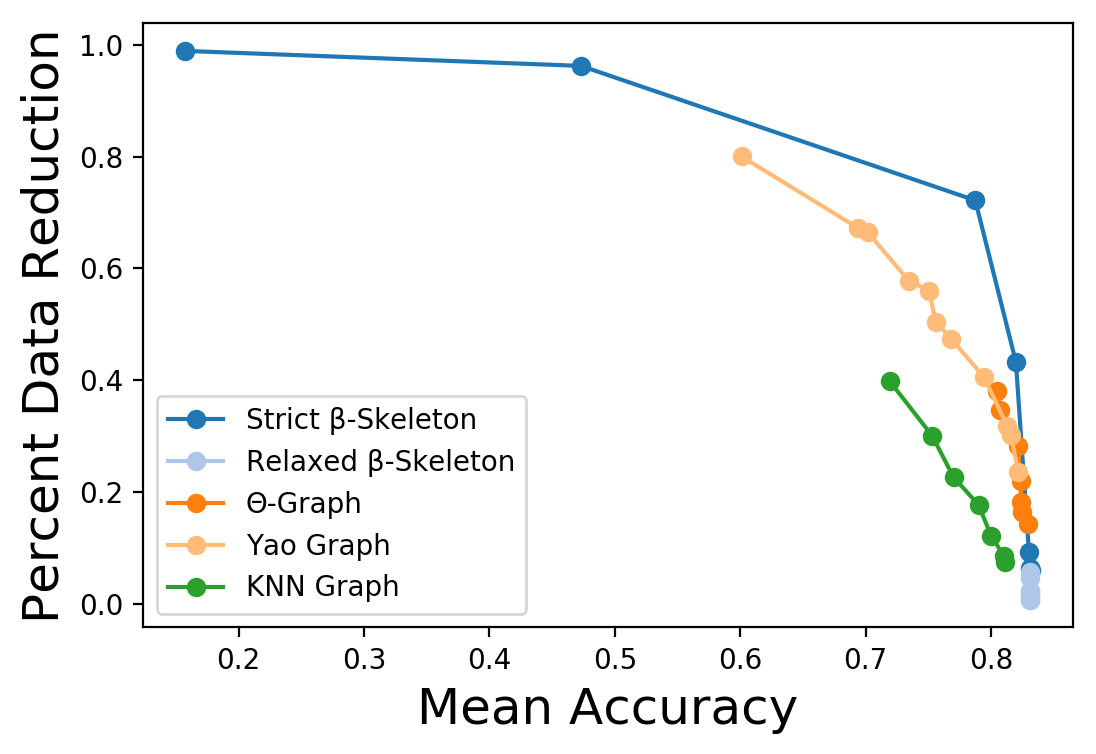
\includegraphics[width=0.48\linewidth]{figs/chap7/pareto_letters.png}
    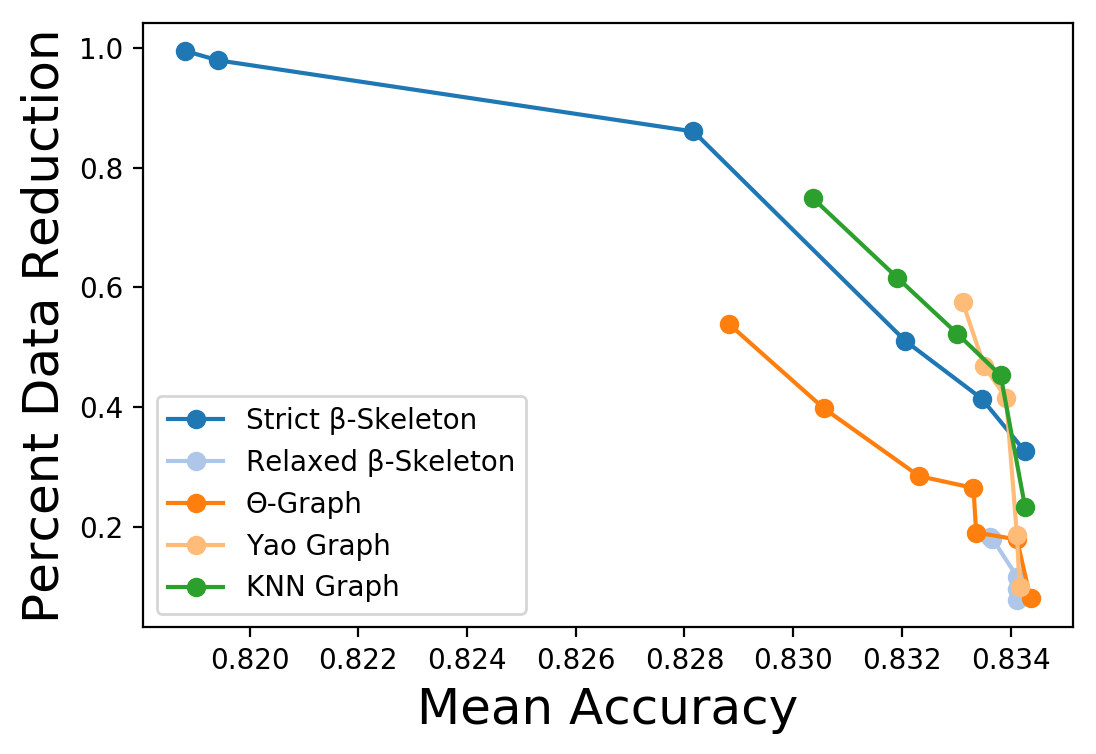
\includegraphics[width=0.48\linewidth]{figs/chap7/pareto_sbo.png}
    \caption[Trade-off analysis of graphs for SVM classification]{Analysis of five graphs for two classification datasets.
    %
    Left: For the SVM evaluation, we report a Pareto front over the handwritten dataset.
    %
    Right: We similarly report results for the station blackout dataset.}
    \label{fig:graph_svm}
\end{figure}

\section{Conclusion}
We have presented three different methods for evaluating the applicability of the various proximity graphs to various problems that arise in data analysis and visualization.
%
First, we took the approach of identifying what we deemed to be important characteristics of a proximity graph, generically speaking.
%
We then evaluated these five quality measures in aggregate over each family of graphs before presenting a concise comparison of the optimal settings in the bar charts of Figure~\ref{fig:graph_quality}.
%
The preliminary analysis was performed by using plots, such as the heatmaps shown in Figure~\ref{fig:teaser}.
%
We then evaluate the same parameter settings and graphs on two specific applications.

We performed a similar analysis on these two applications, in which we first tuned the parameters of each graph before presenting the optimal settings for a side-by-side comparison of the different families of graphs.
%
It is is worth noting that there is not one clear winner among all the applications.
%
That is, different parameterizations of each graph performed better in different situations, and although the strict $\beta$-skeleton was able to outperform the others in the SVM case, the Yao graph could be seen as more stable for the topology case.
%
Additionally, the Yao graph seems to be a good compromise between speed and accuracy since we know the strict $\beta$-skeleton does not scale as well as any of the other proximity graphs to large datasets.

Rather than presenting a comprehensive and unanimous decision about graph selection, we instead present a sampling of different tests and qualities to consider when using such graphs.
%
This study should provide motivation and a template for future studies that rely on such graphs to critically evaluate the desirable characteristics and how they best align with needs of the application.
%
This study represents the kinds of questions that we should be asking of our underlying data structures in general.
%
By identifying a connection between these graphs, providing an efficient and common API, and establishing a baseline for comparison, we hope to inspire others to evaluate the applicability of one or more of these graphs to their needs and also to inspire further explorations pursuing questions raised, but not answered by this work.